\documentclass[a4paper,10pt, english]{report}% norsk istedefor english
%\usepackage{ucs}
\usepackage[utf8]{inputenc}%utf8x
\usepackage[T1]{fontenc}
\usepackage{babel,graphicx,subfigure,epsfig}%,uioforside}%,babel hvis norsk
\usepackage{amssymb,psfrag,amsmath,wick}
\usepackage{wrapfig}
\usepackage{color}  
\usepackage[pdftex]{hyperref}

\newcommand{\be}{ \begin{equation}}
\newcommand{\ee}{ \end{equation}}
\newcommand{\mc}{ \mathcal }
\newcommand{\bra}[1]{\langle #1|}
\newcommand{\ket}[1]{|#1\rangle}
\newcommand{\braket}[2]{\langle #1|#2\rangle}
\newcommand{\beq}{\begin{eqnarray}}
\newcommand{\eeq}{\end{eqnarray}}
\newcommand{\ds}{\displaystyle{\not}}
\newcommand{\bsp}{\begin{split}}
\newcommand{\eesp}{\end{split}}

%\title{AB INITIO STUDIES OF INFINITE MATTER}
%\author{Johannes Rekkedal}
\date{}

\begin{document}
\input frontpage.tex
%\maketitle
%\fysikkforside{}
%\uioforside[inst = Department of Physics]
% maa kompilere med latex istedefor pdflatex for at uioforside 
%skal virke
\pagenumbering{roman}
\tableofcontents
\clearpage
%\listoffigures
%\listoftables


\pagenumbering{arabic}
\chapter{Introduction}
\label{introduction}

\section{Historical Background}

In order to make useful progress the equations must be solved numerically. 
About 2400 years ago, the Greek philosopher Anaxagoras invented the
idea that matter could be devided into infinitly small parts;
\emph{spermata}. 
This concept was expanded a few years later by
Democritus, who believed matter was composed of tiny particles of
finite size or mass. He called the invisible particles of matter
\emph{atoms}; which in greek means 'undevidable'. 
No experimental techniques needed to test the atomic
hypotheses existed at the time, and there was no advance in the
understanding of atoms for more than 2000 years! 

\subsection*{Discovery of the Atom}

In 1807, John Dalton postulated that atoms of each element had a
unique mass. Dalton's atomic theory contained a simple prediction for
the case where two elements combine to form two different compounds;
\emph{The Law of Multiple Proportions}. (For example, 16 g of oxygen, O,
combines with 12 g of carbon, C, to form carbonmonoxide, CO, and
32 g of O combines with 12 g of C to form carbondioxide, CO$_2$).
%
\newline
%
A great leap in the understanding of the structure of matter was made
in 1811 by Amedeo Avogadro. Avogadro correctly hypothesized that the
particles of a gas were small compared to the distance between the
particles. He determined that these particles were often made up of
more than one atom; \emph{molecules}. This important result is the
basis for the \emph{Ideal Gas Law}, and the discovery provided a
systematic method for measurement of the atomic mass numbers.

\subsection*{The Periodic Table}

In 1869, Dmitri Mendeleev made the first classification of the
elements. The elements were ordered with increasing atomic mass
number, and placed in several columns according to their chemical
properties. Mendeleev discovered some gaps, that made him to correctly
predict the existance of undiscovered elements!

\subsection*{Discovery of the Electron}

A type of radiation, called \emph{cathode rays}, was observed to be
emitted from metallic surfaces when voltage was applied. At the end of
the 19$^{th}$ century there was much speculation about the fundamental
properties of the cathode rays. One school of thought held the belief
that cathode rays were particles, while the other school believed it
was a wave-phenomenon. In 1897, Joseph John Thomson preformed a
definitive set of experiments that proved that cathode rays had
a particle behavior. Thomson developed the necessary technique to
observe the deflection of chatode rays in an electric field. This led
to the interpretation of chatode rays as charged particles;
\emph{electrons}.

\subsection*{Measurement of the Electric Charge}

In 1909, Robert Millikan made the first accurate measurement of the
electron charge. \emph{The Millikan Oil-Droplet Experiment} was
performed by spraying tiny droplets of oil between two conducting
plates. By switching the electric field between the two plates on and
off, Millikan was able to accuratly estimate the electron charge. The
result of numerous measurements by Millikan, was that the charge was
allways an integer multiple of $1.6 \cdot 10^{-19}C$.
Figure \ref{oil_droplet} illustrates the forces acting on the
oil-droplet.

\begin{figure}[hbtp]
\begin{center}
  \epsfig{file=Introduction/oil_droplet.eps, height=5cm}
  \caption{
    Forces on an oil-droplet in: \newline
    \hspace*{1.5cm}
           a) Free fall          \newline
    \hspace*{1.5cm}
	   b) Electric field     \newline
    (G=Gravitation, D=Drag, E=Electric force)
  }
  \label{oil_droplet}
\end{center}
\end{figure}

His results were systematically low by about 4\% due to inaccurate
knowledge of the coefficient of viscosity. \newline
The electron charge is -e,
where $e = 1.602 \cdot 10^{-19}C$. All free particles are observed to
have values of electric charge equal to an integer times the
fundamental charge e:

\begin{equation*}
  q=n e
\end{equation*}

where the integer $n=\dots,-1,0,1,\dots$ is the electric charge
\emph{quantum number}.

\subsection*{The Nucleus}

In 1912, Ernest Rutherford and his associates discovered that the
positive charge of the atom is concentrated in a \emph{nucleus}. The
charge of the $\alpha$ particle, discovered by Becquerel, was
determined to be $2e$, and the mass of the $\alpha$ particle was
determined to be about four times the mass of the hydrogen
atom. \newline
A new particle with zero electric charge was discovered by bombarding
beryllium atoms with $\alpha$ particles. James Chadwick showed that
the new particle, the \emph{neutron}, had mass nearly equal to that of
the \emph{proton}.

\subsection*{The Bohr Model of the Atom}

In 1913, Niels Bohr made the first qunatitatively successful model of
the atom. Inspired by the work of Rutherford, Bohr made a planetary
model of the atom; with electrons moving in circular orbits about the
nucleus. This model may seem quite simple in retrospect, but for the
time it was a great advancement of science. In addition to the
classical circular orbits, the second part of Bohr's atomic model
contains a bold hypothesis of new physics. The new physics recognizes
that \emph{angular momentum} is \emph{quantized}; it can take only
certain values:

\begin{equation*}
  L = mvr = n \hbar
\end{equation*}

where $n$ is a positive integer. Solving the energy equations result
in orbits of radius:

\begin{equation*}
  r_n = \frac{n^2\hbar^2}{mke^2}
\end{equation*}

where the \emph{Bohr radius}

\begin{equation*}
  a_0 \equiv r_1 = \frac{\hbar^2}{mke^2} \approx 0.053 nm
\end{equation*}

is in the correct order of magnitude for the size of the atom!

{\bf Planc }





%               The Two First Excited states of Helium
\subsection{The Two First Excited states of Helium}

We will not make any calculations regarding exited states in this
thesis, but it is a really important issue in quantum mechanics. The
ground state energy does not tell much about the 
chemical properties of the atom on its own. Therefore good
approximations of the exited states are needed. Also, when discussing
different numerical approaches for solving the many body-problem,
including linear combinations of exited states may greatly improve
some original approximation to the ground state. Furthermore,
understanding how we include exited states is important for fully
understanding the application of the Slater determinant.
\newline
%
\newline
The state of helium with the $1s$ and the $2s$ orbitals occupied
with one electron each. 








The construction of the
periodic table in the second half of the $19^{\mathrm{th}}$ century
was based on the chemical properties of the different atoms. These
properties were not understood until the development of quantum
mechanics. The electrons are filled from the energetically lowest
orbitals. In the $s$ orbitals only two electrons of different
spins are allowed. Disregarding electron repulsion this would imply
that twice the energy is needed in removing an electron from ground
state helium than from the ground state hydrogen. This due to the 
double electric charge of the helium nucleus. The ionization energy of
hydrogen is $13.60 eV$ and the ionization energy of helium is $24.58
eV$ (ref. \cite{atkins2003}). The electron repulsion thus reduce the
ionization energy by almost $10\%$.
\newline
%
\newline
The early development of quantum theory may be summarized through the
four postulates of quantum mechanics.


%*************** The Postulates of Quantum Mechanics **************
%*
%*
\section{The Postulates of Quantum Mechanics}

A common formulation of quantum mechanics is by means of linear
algebra. In this formulation every state is represented as a (usually
infinite dimensional) complex vector, and an operator is represented
as a complex, linear and hermitian matrix. 
The postulates of quantum mechanics fall naturally into two sets: the
first three, which tell us how the system is depicted at a given time,
and the fourth, which specifies how this picture changes with time. 
\newline

%*                     The First Postulate                              *
%\subsection{The First Postulate}

{\bf \large Postulate 1}
\emph{
The state of a quantum mechanical particle is described by a vector
$\Psi$ in a Hilbert space ${\cal H}$. All the possible states of the
particle are ${\cal H}$ except the zero vector.
\newline
}

The first postulate states that a particle is described as a vector in
the Hilbert space. So a particle with finite degrees of
freedom $\mathbf{x}$ and $\mathbf{p}$ in classical
mechanics, now has infinite degrees of freedom. 
\newline

%*                     The Second Postulate                              *
%\subsection{The Second Postulate}

{\bf \large Postulate 2}
\emph{
Every observable are represented by an Hermitian linear operator in
${\cal H}$. For every classical dynamical variable
$\omega(\mathbf{x},\mathbf{p})$ there is a corresponding quantum
mechanical operator $\Omega$  obtained by operator substitution of the
fundamental position and momentum operators $\mathbf{X}$ and
$\mathbf{P}$, respectively: 
}
%
\begin{equation*}
  \Omega(\mathbf{X},\mathbf{P}) = \omega(\mathbf{x} \to
  \mathbf{X},\mathbf{p} \to \mathbf{P})
\end{equation*}
%
\emph{
The components of $\mathbf{X}$ and $\mathbf{P}$ are operators defined
through the fundamental commutation relation
}

\begin{equation*}
  \left[ X_i, P_j \right] = i \hbar \delta_{ij}
\end{equation*}

The second postulate tell us how to to move from the classical to the
quantum mechanical picture. The observables (or measurable quantities)
are defined through an operator. This operator may be obtained by
simple substitution of the position and the momentum of the
corresponding classical observable.
\newline

%*                     The Third Postulate                              *
%\subsection{The Third Postulate}

{\bf \large Postulate 3}
\emph{
The only possible values obtainable in an (ideal) measurement of an
observable $\Omega$ are its eigenvalues $\omega_n$. Each have a
probability
}
%
\begin{equation*}
  P(\omega_n) = \frac{\int \Psi^* \Phi_n }{\int \Psi^* \Psi }
\end{equation*}
%
\emph{
with $\Phi_n$ the eigenfunction corresponding to the eigenvalue
$\omega_n$. Immediately after a measurement the state collapses into
$\Phi_n$.
}
\newline

The third postulate tells what may be extracted from the quantum
mechanical picture by means of measurements. Note that the eigenvalues
may either have a continuous spectrum or be \emph{quantized}.
\newline


%*                     The Fourth Postulate                              *
%\subsection{The Fourth Postulate}

{\bf \large Postulate 4}
\emph{
The time development of the quantum state $\Psi$ is given by the time
dependent Schr\"odinger equation,
}

\begin{equation*}
  \hat{H} \Psi(\mathbf{x},t) = i\hbar \frac{\delta}{\delta
  t}\Psi(\mathbf{x},t) 
\end{equation*}

The fourth and final postulate defines the Schr\"odinger
equation. This equation describes how the quantum mechanical state
evolve in time.
\newline




 % introduction.tex
\chapter{The Second Quantization}
\label{chapsecondq}

Nuclear physics is about many-particle systems, the need for interparticle
potentials has to be accounted for when trying to describe 
 such systems. The interparticle potentials have to be implemented in the
many-particle Schr\"odinger equation.
A direct solution of the schr\"odinger equation in configuration space is impractical \cite{fetter}. 
It is necessary to resort to other techniques such as the second 
quantization.\\

The system studied in this text consists of nucleons which belong to the 
types of particles called fermions. Fermions are particles with half 
integer spin. 
A system of fermions is described by an antisymmetric wave function, these particles obeys the Pauli principle which states that two identical 
fermions can not occupy the same single particle state.\\

In most of the cases of interest, as is also the case in this text, the Hamiltonian 
takes the form 

\be
H=\sum_{k=1}^NT(x_k)+\frac{1}{2}\sum_{k \neq l =1}^N V(x_k,x_l).
\label{hamfirst}
\ee  

Where $T$ is the kinetic energy and V is the potential energy of interaction
between the particles, while $x_k$ denotes the coordinates of particle $k$.
The potential energy term represents the interaction between every pair of 
particles, counted once which account for the factor of $\frac{1}{2}$ 
\cite{fetter}.

\section{Creation and annihilation operators}

The interpretation of occupation of the antisymmetric many-body fermion
states allows to introduce the two operators $a^\dagger_\alpha$ and 
$a_\alpha$, which creates and annihilates a particle in the single particle 
state $\alpha$.

\be
\begin{split}
& a^\dagger_\alpha \ket{0}=\ket{\alpha}\\
& a_\alpha \ket{\alpha}=\ket{0}
\end{split}
\ee 

The algebra of these operators depends on whether the system under 
consideration is a system of bosons or a system of fermions. If it consists of bosons the operators obey the commutation relations

\be
\begin{split}
& [a_k,a^\dagger_{k'}]=\delta_{k,k'}\\
& [a_k,a_{k'}]=[a^\dagger_k,a^\dagger_{k'}]=0.
\end{split}
\ee

While in the fermion case they obey the anti commutation relations

\be
\begin{split}
& \{a_k,a^\dagger_{k'}\}=\delta_{k,k'}\\
& \{a_k,a_{k'}\}=\{a^\dagger_k,a^\dagger_{k'}\}=0
\end{split}
\ee

With these expressions for the commutations and anti commutations 
between the creation and annihilation operators the Hamiltonian can be 
reshaped to the form in Eq. \eqref{hamiltoniansec}.

\be
H=\sum_{ik} T_{ki}a^\dagger_ka_i + \frac{1}{2}\sum_{ijkl}V_{ijkl}a^\dagger_i
a^\dagger_ja_la_k.
\label{hamiltoniansec}
\ee

When the operators in the second quantization are non-relativistic and 
conserve the particle number, there should be an equal amount of creation
and destruction operators in the Hamiltonian. A second quantized one particle 
operator, an operator that acts on one particle a time is written as in 
Eq. \eqref{onesec}

\be
F=\sum_{\alpha,\beta}\bra{\alpha}f\ket{\beta}a^\dagger_\alpha a_\beta,
\label{onesec}
\ee 

and a two particle operator is written in the form as in Eq. \eqref{twosec}

\be
V=\frac{1}{2}\sum_{\alpha\beta\gamma\delta}\bra{\alpha\beta}v\ket{\gamma\delta}
a^\dagger_\alpha a^\dagger_\beta a_\delta a_\gamma.
\label{twosec}
\ee





\section{Wicks Theorem}
\label{wicksteorem}
A normal ordered second quantized operator is defined as an operator whose 
all annihilation operators stands to right of all the creation operators. 
It is in some manner easier to calculate when the annihilation operators are
placed to the right.
Wicks theorem describes a fast method to put the annihilation operators to
the right of the creation operators, by using the anti commutation rules
for these operators. Before introducing Wicks theorem some definitions should
be introduced like the normal product of operators and contractions of 
operators. 

Given a product 

\beq
XYZ\cdots W
\eeq

of creation and annihilation operators, the normal product is defined as 

\beq
N(XYZ \cdots W),
\eeq
 
where all the destruction operators stand to the right of the creation 
operators. Thus as an example let us study the cases

\be
N(a^\dagger_\alpha a_\beta)=a^\dagger_\alpha a_\beta
\ee

and

\be
N(a_\alpha a^\dagger_\beta)=\pm a^\dagger_\beta a_\alpha,
\ee

where the minus sign yields for operators acting only on fermions , and the plus 
sign yields for operators acting on  bosons. 

One of the properties of a normalized product of operators is that the
ground state expectation value of the product is zero since the destruction 
operator annihilates the ground state. 

A contraction of two operators $XY$ is defined as it's  expectation value 
regarding the ground state.

\be
\wick{1}{<1a_\alpha >1a^\dagger_\beta}=\bra{0}a_\alpha a^\dagger_\beta\ket{0}=\bra{0}\delta_{\alpha\beta}-a^\dagger_\beta a_\alpha \ket{0}=\delta_{\alpha\beta}
\label{contraction}
\ee  

By having defined the normal product and the contraction we are now ready to 
state Wicks theorem which says that a product of randomly oriented 
creation and annihilation operators can be written as the normal product of
these operators plus the normal product of all possible contractions.

\be
XYZ\cdots W=N(XYZ\cdots W) + \sum^{all \, possible}_{contractions} N(XYZ \cdots W)
\label{wicks}
\ee

As a remark, in this theorem only fermions has been considered.

The proof of this theorem can be found in almost all books that treat 
quantum field theory or quantum theory of many particles such as \cite{heinonen}.



\section{The Particle-Hole Formalism}
\label{particlehole}
In a theory of many particles, there is often more convenient to use another
state as reference state rather than the vacuum state. This reference state
should be a stable state. The normal ordering will then be altered from the one given above for the true vacuum state. That is our new vacuum state
$\ket{\Phi_0}=a^\dagger_ia^\dagger_j \cdots$. A somehow new definition of the
creation and destruction operators is needed. The operators will now create and 
annihilate holes and particles. The definition of a hole is a one particle
state that is occupied in the reference state $\ket{\Phi_0}$, while a 
particle state is one particle state that is not occupied in $\ket{\Phi_0}.$
This new nomenclature is easily understood when considering that a "hole" is
created when an originally occupied state is acted upon by an annihilation 
operator such as $a_i.$ A "particle" is created when an unoccupied state is
acted upon by a creation operator. These operators that destroy and create 
holes and particles are called quasiparticle 
operators. A q-annihilation operator annihilates holes and particles, 
while a q-creation operator creates holes and particles. 

A normal ordered product of quasiparticle operators would then be defined as
a product where all the quasiparticle destruction operators stand to the right
of all the quasiparticle creation operators. This definition of the normal 
ordered product changes the analysis of Wick's theorem a bit. The only
contractions that contribute are the ones where a destruction operator 
stands to the left of a creation  operator, there are two ways this can 
happen

\be
\begin{split}
& \wick{1}{<1a_i^\dagger>1a_j}=a^\dagger_i a_j-N(a^\dagger_ia_j)=a^\dagger_i
a_j+a_ja^\dagger_i=\delta_{ij}\\
& \wick{1}{<1a_i>1a^\dagger_j}=a_ia^\dagger_j-N(a_ia^\dagger_j)=a_ia^\dagger_j+a^\dagger_ja_i=\delta_{ij}
\label{normalhole}
\end{split}
\ee
 
That is if $i$ defines a hole state in Eqs. \eqref{normalhole}.

As an example, consider normal ordering of a two particle Hamiltonian, as 
the one in Eq. \eqref{twoham}.

\be
\hat H = \sum_{pq}\bra{p}h\ket{q}a^\dagger_p a_q + \frac{1}{4}\sum_{pqrs}
\bra{pq}V\ket{rs}a^\dagger_p a^\dagger_qa_sa_r
\label{twoham}
\ee


The one particle part can be written as 

\be
\sum_{pq}\bra{p}h\ket{q}N(a^\dagger_p a_q)+\sum_{i\in hole}\bra{i}h\ket{i}
\ee

While the two particle part would be rewritten as 

\be
\begin{split}
& \frac{1}{4}\sum_{pqrs} \bra{pq}V\ket{rs}a^\dagger_p a^\dagger_pa_sa_r=\\
& \frac{1}{4}\sum_{pqrs} \bra{pq}V\ket{rs}N(a^\dagger_p a^\dagger_q a_s a_r)
+\sum_{ipq}\bra{pi}V\ket{q i}N(a^\dagger_pa_r)+\frac{1}{2}\sum_{ij}\bra{ij}V\ket{ij}
\label{normH}.
\end{split}
\ee

After some tedious work, for the entire calculation see \cite{sjefer}.
After the equal sign in Eq. \eqref{normH} the letters $p,q,r,$ and $s$ indicate 
both hole and particle states, while the letters $i$ and $j$   indicate hole states.
The entire Hamiltonian is then written as

\be
\begin{split}
& \sum_{pq}\bra{p}h\ket{q}N(a^\dagger_p a_q)+\sum_i\bra{i}h\ket{i}+
\frac{1}{2}\sum_{ij}\bra{ij}V\ket{ij}+\\
& \frac{1}{4}\sum_{pqrs} \bra{pq}V\ket{rs}N(a^\dagger_p a^\dagger_q a_s a_r)
+\sum_{ipq}\bra{pi}V\ket{qi}N(a^\dagger_p a_q)
\label{normalham}
\end{split}
\ee

Where $p,q,r,$ and $s$ still run over all states, $i$ and $j$ over hole states only.

\chapter{Perturbation Theory}

The many body Schr\" odinger equation is rather difficult to solve. 
Even a two body problem is a rather complicated system to solve, that is why
we have to come up with approximated methods. Usually the Hamiltonian gets 
separated in an unperturbed part and a perturbed part, The perturbed part is
the one which considers the interactions between the particles. 

\be
H\Psi=(H_0 +V)\Psi=E\Psi.
\ee

$H_0$ is the unperturbed Hamiltonian, which is a one particle operator, 
which in most of the problems governing nuclear physics is a harmonic 
oscillator Hamiltonian. Then $H_0=E_{kin} + U_{H.O}$ and $V = V-U_{H.O}.$
Where $E_{kin}$ is the kinetic energy and $U_{H.O}$ is the harmonic oscillator potential. 
Obviously the difference $V-U_{H.O}$ should be small enough so that
 threating $V$ as a perturbation is valid. The exact result is independent of the one particle potential $U$, but 
in an approximated calculation it is possible that the results depend on the one particle potential that is included in
the calculations. The eigenfunctions, $\phi_i$ are taken as a basis for the expansion of the eigenfunction $\Psi$


\be
\ket{\Psi}=\sum_{i=1}a_i\ket{\phi_i}
\ee

It is common practice to divide the space in a model space and an excluded space, to simplify the calculations. By doing this we define 
two projection operators, that we will meet again later. These projection operators are denoted by a $P$ and a $Q.$ The $P$ operator projects
the complete wavefunction onto the model space 

\be
P\ket{\Psi}=\ket{\Psi_M}.
\ee


While $Q$ is the complimentary projector operator and projects the complete wavefunction to the excluded state $\ket{\Psi_Q}.$ 

\be
\begin{split}
P=\sum_{i=1}^d \ket{\phi_i}\bra{\phi_i}\\
Q=\sum_{i=d+1}^N \ket{\phi_i}\bra{\phi_i}\\
\end{split}
\ee
The projection operators satisfy the properties

\be
\begin{split}
P^2=P\\
Q^2=Q\\
PQ=QP=0\\
P+Q=1
\end{split}
\label{projectionopprop}
\ee

Since $e_k$ are the eigenvalues of the unperturbed Hamiltonian $H_0$, we obtain that 

\be
(E-e_j)a_j=\bra{\phi_j}V\ket{\Psi}.
\label{differense}
\ee

By using this relation we find that the entire wavefunction $\ket{\Psi}$ can be written as

\be
\ket{\Psi}= \sum_{i=1}^d a_i\ket{\phi_i} + \sum_{i=d+1}^N\frac{\ket{\phi_i}\bra{\phi_i}V\ket{\Psi}}{E-e_i}=\sum_{i=1}^da_i\ket{\phi_i} + \frac{QV}{E-H_0}\ket{\Psi}= P\ket{\Psi} + \frac{QV}{E-H_0}\ket{\Psi}
\ee

If we now define a wave operator which projects the model space onto the complete wavefunction $\Omega\ket{\Psi_M}=\ket{\Psi}$ we find it to be


\be
\Omega(E)=1 + \frac{Q}{E-H_0}V\Omega(E)
\ee

If we now use the wave operator in Eq \eqref{differense} we get 

\be
(E-e_j)a_j=\bra{\phi_j}V\Omega\ket{\Psi_M}=\sum_{k=1}^d\bra{\phi_j}V\Omega\ket{\phi_k}a_k
\ee

which is equivalent to 

\be
[H_0 + V\Omega(E) -E]\Psi_M=0.
\ee


If we define an effective interaction 

\be
\mathcal V(E)=V\Omega(E)
\ee

we get an integral equation, 

\be
\mathcal V(E)=V + V\frac{Q}{E-H_0}\mathcal V(\Omega),
\label{effektivvv}
\ee

for the effective interaction, which is dependent on the energy $E$. 
Eq. \eqref{effektivvv} can be solved by iteration, where we by using $V$ as
a first guess find that

\be
\begin{split}
&\mathcal V(E)=V + VQ\frac{1}{E-H_0}QV +VQ\frac{1}{E-H_0}QVQ\frac{1}{E-H_0}QV
+\\
& VQ\frac{1}{E-H_0}QVQ\frac{1}{E-H_0}QVQ\frac{1}{E-H_0}QV + \cdots
\end{split}
\ee

This can be solved analytically by observing that the sum resembles a 
geometric sum. 

\be
\begin{split}
\mathcal V=V + VQ\frac{1}{E-H_0-QVQ}QV\\
\equiv PVP + PVQ\frac{1}{E-QHQ}QVP
\end{split}
\ee


\section{Time dependent perturbation theory}


When doing time dependent perturbation theory we have to define the time 
evolution propagator $U(t,t')$, the time evolution operator evolve a state 
$\Psi(t')$ at time $t'$ to state $\Psi(t)$ at 
time $t$. 

\be
\Psi(t)=U(t,t')\Psi(t')
\ee

The wavefunctions satisfy the time dependent Schr\" odinger equation, 

\be
\begin{split}
&i\hbar \frac{\partial}{\partial t}\Psi(t)=H\Psi(t)\\
&i\hbar \frac{\partial}{\partial t}\Psi(t)=i\hbar \frac{\partial}{\partial t}U(t,t')\Psi(t'),
\end{split}
\ee

which yields that the time evolution operator satisfy Schro\" dinger equation. The solution is

\be
U(t,t')=e^{-iH(t-t')/\hbar}.
\ee


This form of the time evolution operator gives right away the properties one would expect of an
operator of this kind

\be
\begin{split}
&U(t,t)=1\\
&U(t',t)U(t,t')=1\\
&U(t,t')U(t,t')^\dagger=U(t,t')^\dagger U(t,t')=1\\
&\rightarrow U(t',t)=U(t,t')^\dagger=U(t,t')^{-1}\\
&U(t_1,t_2)U(t_2,t_3)=U(t_1,t_3)
\end{split}
\ee


By use of Thouless theorem \cite{thouless}, exact eigenstates can be constructed
through the action of the time-development operator.  In the present approach
the time $t$ will be rotated by a small angle $\epsilon$, our time is complex. 

The eigenstate can the be written as

\be
\frac{\ket{\psi_i}}{\braket{\phi}{\psi_i}}=\substack{lim\\ \epsilon \rightarrow 0}\, \substack{lim\\t'\rightarrow\\-\infty(1-i\epsilon)}
\frac{U(t,t')\ket{\phi}}{\bra{\phi}U(t,t')\ket{\phi}},
\label{eigenstatefortime}
\ee

where $\ket{\psi_i}$ is the lowest state of $H$ with $\braket{\phi}{\psi_i}\neq
0.$ This relationship is very useful in calculating the ground state energy
shift $\Delta E_0.$

If our unperturbed Hamiltonian gives the energy $E_0$ while acting on the
unperturbed state $\ket{\phi}$, and our total energy is $E$ the ground state
energy shift is given by

\be
\begin{split}
&\Delta E_0=E-E_0=\frac{\bra{\phi}V\ket{\psi}}{\braket{\phi}{\psi}}\\
&=\substack{lim\\ \epsilon \rightarrow 0^+}\substack{lim \\t'\rightarrow \\
 -\infty(1-i\epsilon)}\frac{\bra{\phi}VU(0,t')\ket{\phi}}{\bra{\phi}U(0,t')\ket{\phi}}
\label{energyshift1}
\end{split}
\ee

To evaluate this as a perturbation, we have to expand the time evolution
operator $U(t,t')$. This is most conveniently if it is done in the interaction
picture. Which will be explained slightly here, \cite{shankar94} and
\cite{sakurai} give a more thoroughly explanation of the interaction picture. 
The interaction picture can be understood as an intermediate between the Schr\" odinger picture and the Heisenberg picture. In the Schr\" odinger picture the 
operators are time independent while the state evolves with time. It is all
contrary in the Heisenberg picture where the operators now are time dependent
and the state is time independent.
In the interaction picture both the state vectors and the operators are time
dependent, however their time dependencies are somewhat different.

A state vector in the interaction picture is defined as

\be
\ket{\psi_I(t)}=e^{iH_{0,S}t/\hbar}\ket{\psi_s(t)}
\ee


where the letter $S$ stands for the schr\" odinger picture. The operators in the interaction picture is defined as

\be
A_{I}(t) = e^{i H_{0,S} t / \hbar} A_{S}(t) e^{-i H_{0,S} t / \hbar}. 
\ee

$H_0$ is still the unperturbed Hamiltonian. The time evolution of the operators is given by 

\be
i\hbar\frac{d}{dt}A_I(t)=\left[A_I(t),H_0\right].\; 
\ee



By using the definition of one particle and two particle operators from chapter
\ref{chapsecondq}, our Hamiltonian can be written as in Eq.
 \eqref{hamiltoniansec}


\be
H=\sum_{k} \epsilon_{k}a^\dagger_ka_k + \frac{1}{2}\sum_{ijkl}V_{ijkl}a^\dagger_i
a^\dagger_ja_la_k.
\ee

To find the time evolution of  the Hamiltonian it suffices to find the time
evolution of the creation and annihilation operators $a^\dagger$ and $a.$
Using the commutator we find that

\be
\left[a^\dagger_k,H_0\right]=-\epsilon a^\dagger_k(t)
\ee

thus we obtain the time dependence of the creation and destruction operators

\be
\begin{split}
& a^\dagger(t)_k=a^\dagger_ke^{i\epsilon_kt/\hbar}\\
& a(t)_k=a_ke^{-i\epsilon_kt/\hbar}
\end{split}
\ee

I will now transform the schr\" odinger equation to the interaction picture

\be
\begin{split}
&\psi_I(t)=e^{iH_0t/\hbar}\psi(t)\\
&=e^{iH_0t/\hbar}U(t,t')e^{-iH_0t'/\hbar}e^{iH_0t'/\hbar}\psi(t')\\
&=U_I(t,t')\psi_I(t')
\end{split}
\label{itertimeop}
\ee

By differentiating Eq. \eqref{itertimeop} with respect to time $t$ we find

\be
\frac{\partial}{\partial t}U(t,t')=VU(t,t')
\ee

When we have found how the time evolution operator we may also find the 
perturbartive expansion of the time evolution operator. The solution to the differential equation is 

\be
U(t,t')=1 +\left(\frac{-i}{\hbar}\right) \int_{t'}^tdt_1V(t_1)U(t_1,t')
\label{ekspavtidev}
\ee


The number 1 in Eq. \eqref{ekspavtidev} is for satisfying $U(t',t')=1.$
Eq. \eqref{ekspavtidev} can be solved by iteration

\be
U(t,t')=1+\sum_{n=1}^\infty\left(\frac{-i}{\hbar}\right)^n\int_{t'}^tdt_1
\int_{t'}^{t_1}dt_2\cdots \int_{t'}^{t_{n-1}}dt_nV(t_1)V(t_2)\cdots V(t_n)
\ee

Now the above form of the time evolution operator can be inserted into Eq. 
\eqref{eigenstatefortime}, which gives us the perturbative expansion for
calculating the interactions.


\section{Feynman-Goldstone diagrams}

To evaluate Eq. \eqref{eigenstatefortime} we had to define a new operator, called the time ordering operator. The effect of operating this operator on a 
product of operators is to order the operators so the operators with a larger
time argument are placed to the left to those of smaller time arguments. Since we in nuclear physics are dealing with fermions which obey the Pauli exclusion
principle there will be a sign dependency on the number of permutations needed 
in making the arrangement. As an example 

\be
\begin{split}
T\left[A_1(t_1)A_2(t_2)\cdots A_n(t_n) \right]\\
=(-1)^pA_\alpha(t_\alpha)A_\beta(t_\beta) \cdots A_\gamma(t_\gamma)
\end{split}
\ee

If we use time ordering together with the particle hole formalism from section \ref{particlehole}, we will find a new definition of the contraction.
A contraction of two operators will now be defined as

\be
\wick{1}{<1A>1B}=T[AB]-N[AB], 
\ee

Where $N[AB]$ is the normal ordering operator. 
As an example I will derive a contraction 
of two hole operators and a contraction of two particle operators. 
I will first start with a contraction of two hole operators where both 
particles have momenta below $k_F,$ and with $t < t'.$


\be
\begin{split}
&\wick{1}{<1a_h(t)>1a_{h'}^\dagger (t')}=T\left[a_h(t)a_{h'}^\dagger (t')\right]
-N\left[a_h(t)a_{h'}^\dagger (t')\right]\\
&=-a_{h'}^\dagger (t')a_h(t)-a_h(t)a_{h'}^\dagger(t')\\
&=-\left(a^\dagger_{h'}(t')a_h(t)+a_h(t)a_{h'}^\dagger(t')\right)e^{-\frac{i}{\hbar}(\epsilon_ht-\epsilon_{h'}t')}\\
& = -\delta_{h,h'}e^{-\frac{i}{\hbar}(\epsilon_ht-\epsilon_{h'}t')}.
\end{split}
\label{kontrakt1}
\ee

Similarly for particles with momenta above $k_F$ and $t<t'$

\be
\wick{1}{<*a_p(t)>*a_{p'}(t')}=\delta_{p,p'}e^{-\frac{i}{\hbar}\epsilon_p(t-t')}
\label{kontrakt2}
\ee

We have 

\be
\wick{1}{<*a_\alpha(t)>*a_\beta^\dagger(t')}=-\wick{1}{<*a_\beta^\dagger(t')>*a_\alpha(t)}
\ee

\begin{figure}[htp]
\centering
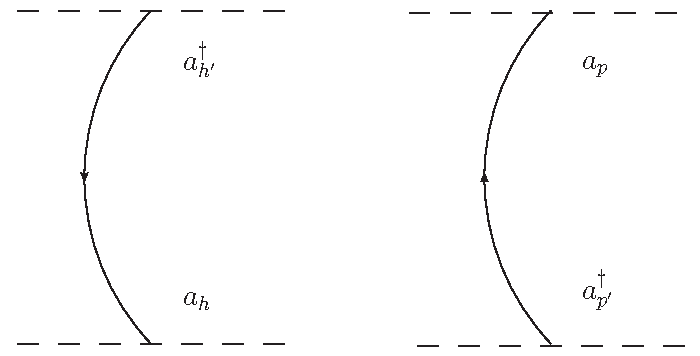
\includegraphics[scale=0.5]{hullpartlinje}
\caption{Diagrammatic representation of the contractions in Eqs. 
\eqref{kontrakt1} and \eqref{kontrakt2} The time is going upward.}
\label{hullpartlinje}
\end{figure}

In Fig (\ref{hullpartlinje}) the two contractions in Eqs \eqref{kontrakt1} 
and \eqref{kontrakt2} are represented diagrammatically, the annihilation 
operator $a_\alpha$ destroys the particle line $a^\dagger_\beta$ creates. The
time is upward.

With the above definitions of time ordering and contractions we are ready to go back to the time evolution operator, it is already in a time ordered 
form.

\be
U(t,t')=\sum_{n=0}^\infty\left(\frac{-i}{\hbar}\right)^n\int_{t'}^tdt_1
\int_{t'}^{t_1}dt_2\cdots \int_{t'}^{t_{n-1}}dt_nT\left[V(t_1)V(t_2)\cdots V(t_n)\right]
\label{tidevolusjon1}
\ee

From  Eq. \eqref{tidevolusjon1} we see that the integral with respect to the time $t_1,t_2 \cdots t_n$ and that there are $n!$ ways to order them, we can again rewrite the time evolution operator in the form



\be
U(t,t')=\sum_{n=0}^\infty\frac{1}{n!}\left(\frac{-i}{\hbar}\right)^n\int_{t'}^tdt_1
\int_{t'}^{t}dt_2\cdots \int_{t'}^{t}dt_nT\left[V(t_1)V(t_2)\cdots V(t_n)\right]
\label{tidevolusjon2}
\ee


If we recall that it is the energy shift we want to calculate, we can rewrite Eq. \eqref{energyshift1}



\be
\begin{split}
&\Delta E_0=\substack{lim\\ \epsilon \rightarrow 0^+}\substack{lim \\t'\rightarrow \\
 -\infty(1-i\epsilon)}\frac{\bra{\phi}VU(0,t')\ket{\phi}}{\bra{\phi}U(0,t')\ket{\phi}}\\
&=\sum_{n=0}^\infty\frac{1}{n!}\left(\frac{-i}{\hbar}\right)^n\int_{t'}^tdt_1
\int_{t'}^{t}dt_2\cdots \int_{t'}^{t}dt_n\bra{\phi}T\left[V(t)V(t_1)V(t_2)\cdots V(t_n)\right]\ket{\phi}\\
&\times \frac{1}{\sum_{n=0}^\infty\frac{1}{n!}\left(\frac{-i}{\hbar}\right)^n\int_{t'}^tdt_1
\int_{t'}^{t}dt_2\cdots \int_{t'}^{t}dt_n\bra{\phi}T\left[V(t_1)V(t_2)\cdots V(t_n)\right]\ket{\phi}}.
\end{split}
\label{energyshift2}
\ee

Where $V(t)$ in the numerator in  Eq. \eqref{energyshift2} is put into to 
the time ordering operator. 
To evaluate the integrals in the numerator and the
denominator we have to use wicks theorem, wicks theorem with time ordering
will be slightly modified from the first version in section \ref{wicksteorem}. Wicks theorem states now that 

\be
\begin{split}
&T\left[A(t_1)B(t_2)C(t_3) \cdots Z(t_n)\right]=N\left[A(t_1)B(t_2)C(T_3) \cdots Z(t_n)\right]\\
&+ \sum_{1\, contraction}N\left[A(t_1)B(t_2)C(T_3) \cdots Z(t_n)\right]+\sum_{2\, contractions}N\left[A(t_1)B(t_2)C(T_3) \cdots Z(t_n)\right]\\
&+ \cdots + \sum_{\substack{contractions\, with\\ all \, operators}}N\left[A(t_1)B(t_2)C(T_3) \cdots Z(t_n)\right]\\
\end{split}
\label{wicktheofortime}
\ee

Since our unperturbed state is the groundstate, which is our reference vacuum state, only the last term in Eq. \eqref{wicktheofortime} survive. We are 
left with the term where all operators are participating in the contractions.

Let us now evaluate the first order contribution to the energy shift in Eq. \eqref{energyshift2}. The only contributing term is $V(t)$ which in 
a second quantized form is $V_{\alpha\beta\gamma\delta}a^\dagger_\alpha(t) a^\dagger_\beta(t) a_\delta(t) a_\gamma(t).$
From wicks theorem we will then have two terms contributing to the energy shift.

\be
\begin{split}
\wick{21}{<*a^\dagger_\alpha(t) <2a^\dagger_\beta(t) >2 a_\delta(t) >*a_\gamma(t)} +
\wick{21}{<*a^\dagger_\alpha(t) <2a^\dagger_\beta(t) >* a_\delta(t) >2a_\gamma(t)} 
\end{split}
\label{forsteordenbidrag}
\ee


The terms in Eq. \eqref{forsteordenbidrag} can be depicted diagrammatically 
as seen in Fig (\ref{forsteordendiagram}).

\begin{figure}[htp]
\centering
%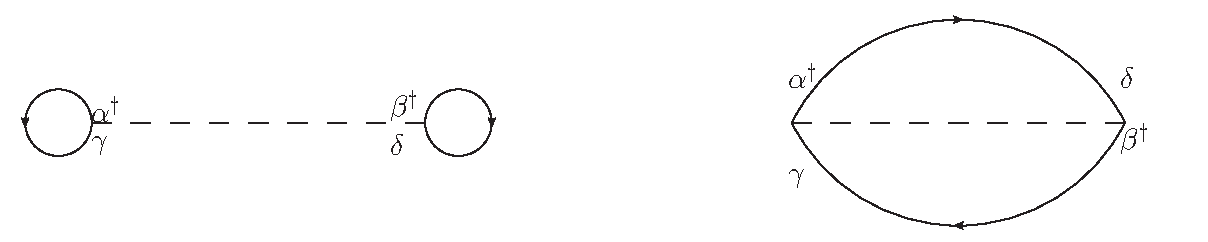
\includegraphics[height=0.8\textheighti]{forsteordendiagram}
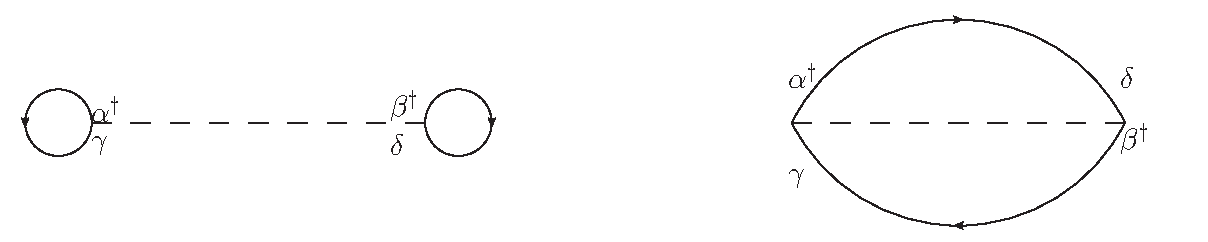
\includegraphics[scale=0.5]{forsteordendiagram}  %[width=1.0\textwidth]{forsteordendiagram}
\caption{Diagrammatic representation of the first order diagram, the diagram to the left depicts the first term in Eq. \eqref{forsteordenbidrag}, the 
diagram to the right depicts the second term in Eq. \eqref{forsteordenbidrag}.}
\label{forsteordendiagram}
\end{figure}

$\alpha, \, \beta, \, \gamma$ and $\delta$ must all be holes, since they are all equal time operators and hence the only contractions which contribute.
The energy shift can now be written as 

\be
\Delta E_0=	 \frac{1}{2}\sum_{\alpha\beta < k_f} \frac{1}{2}(V_{\alpha\beta\alpha\beta}-V_{\alpha\beta\beta\alpha})
\ee

The minus sign comes in, by the "rule" that for every contraction that cross
another contributes with a factor $(-1).$

With the clever invention of the diagrams that depicts the contractions, we are
able to describe every term in the expansion of the time evolution operator as
diagrams. These diagrams are usually called Feynman diagrams or
Feynman-Goldstone diagrams, to honor the inventor.  When presenting all the
terms as diagrams we need some rules to keep track of them. The idea is that we
find a term in the expansion by studying the corresponding diagram. A nice derivation of the diagram
rules can be found in \cite{kuo1981}.  The rules are described in appendix
\ref{diagramregler}. 




 % vlowk.tex
\chapter{The nucleon-nucleon potential}

Since Chadwick discovered the neutron in 1932, understanding the 
nucleon-nucleon interaction has been a main focus for nuclear physicists.
Yukawa \cite{yukawa35} proposed the first significant theory of the nuclear 
force, where a meson is exchanged in the nucleon-nucleon interaction. This 
meson were later to be identified with the pion. The one pion exchange model
turned out to be very useful in explaining nucleon-nucleon scattering data 
and the properties of the deuteron \cite{machleidt2007}. 
Problems arose when multipion exchange were included, and the "pion 
theories" of the 1950's are generally judged to be failures 
\cite{machleidt2007}. 
The reasons for the failure of the theories in the 50's is because of the
then unknown pion dynamics understood by QCD and chiral symmetries, which were not to be used by the nuclear physicists until the 80's. 
The problem of the nuclear force seemed to have been solved by using QCD, however there are still remaining problems such as the nonperturabtive 
character in the low energy regime, where nuclear physicists are working in.

%The nucleon-nucleon potential is highly repulsive in the short distance as can be seen in Fig(\ref{nucleon_pot}), this repulsive "core" is responsible 
%for why it is prohibitive to do ordinary perturbation theory.
%This problem is circumvented by introducing models containing some of the properties of QCD. All of the realistic models treat the long distance part in 
%a similar manner, by one-pion exchange. They are more varying in the intermediate an short distance part. In this text "$N^3LO$" is the mostly used 
%model. It is derived by chiral perturbation theory, which will be explained below.   
%For a description of various models I refer to\cite{machleidt-1994-242}.  

\begin{figure}[htp]
\centering
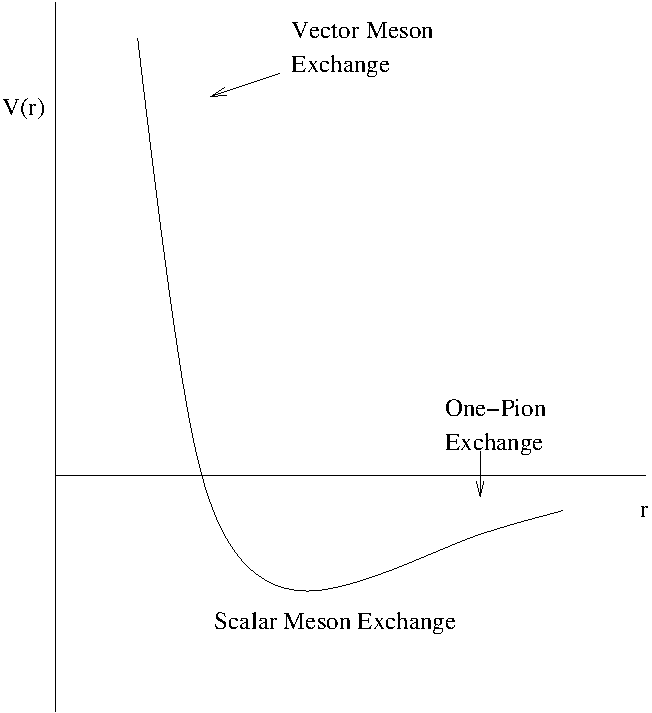
\includegraphics[scale=0.50]{nucleon-nucleon_pot}
\caption{The behavior of the nucleon-nucleon interaction}
\label{nucleon_pot}
\end{figure}

%Fig(\ref{nucleon_pot}) shows the behavior of the nucleon-nucleon interaction, it is repulsive at short distances. 


\section{Chiral Perturbation Theory}

The discovery of QCD and the understanding of effective field theory was a breakthrough for understanding the nucleon-nucleon potential.\\
 QCD is the 
theory of the strong interaction, where the quarks and gluons are treated as the degrees of freedom. 
The principles behind the theory are really simple and 
elegant, the interactions are derived by demanding that the Lagrangian is gauge invariant under SU(3). 
QCD is a non-Abelian field theory which is a consequence of 
the discovery of the three quantum numbers of color. The underlying gauge group is the SU(3) group. QCD is also known for "asymptotic freedom", the force
is weak at short distances but strong, at long distances or at low energies. The consequences of the asymptotic freedom is that the quarks are confined 
into "colorless" objects, called hadrons, and that perturbation theory in the low energy regime is strictly forbidden. As noted earlier nuclear physics 
is in this limit, and diffiulties arise when treating quarks and gluons in the nuclear force. 
The solution is to identify the relevant degrees of freedom, which in the nuclear case are the nucleons, we treat the nucleons as "elementary" particles 
and not a composite of quarks. When identifying the nucleons as the degrees of freedom we have to take in consideration the properties of the quarks,
they will be considered, but hidden in the coupling constants.\\

When constructing an effective field theory from QCD, all the symmetries 
of the Lagrangian should be manifest in the effective Lagrangian. In the case
of QCD, the Lagrangian is invariant under SU(3) transformation. \\
In the limit where the quark masses are zero, the chiral limit, the 
Lagrangian may be separated into a Lagrangian of left and right handed 
fields. The Lagrangian is invariant under left and right handed SU(3) 
transformations in the chiral limit.

We know that the quarks are not massless, but it is not a bad approximation
in the nuclear scale since $m_{u,d,s} \ll m_N$, where $u,d,s$ denotes the 
up, down and the strange quark, while $m_N$ stands for the nucleon mass. 
The remarkable theorem by Emma Noether states that for each symmetry of
the Lagrangian there exists a conserved current. In the case of chiral 
invariance the conserved currents are the left handed and the right handed 
ones. However these two currents can combine to a vector current 
$J^{\mu,b}_V$  and an axial current $J^{\mu , b}_A$. Where 

\be
\begin{split}
& J^{\mu, b}_V=R^{\mu, b} + L^{\mu,b }=\overline q \gamma^\mu \frac{\lambda^b}{2}q \\
& J^{\mu,b}_A=R^{\mu, b} - L^{\mu,b }=\overline q \gamma^\mu \gamma_5 \frac{\lambda^b}{2}q \\
\end{split}
\ee

For each current there is a corresponding charge, Q, which is a generator of $SU(3)_V\times SU(3)_A$, that is conserved.

The conserved charges will in this case be

\be
\begin{split}
& Q^b_V=\int d^3xJ^{0,b} \\
& Q^b_A=\int d^3xJ^{0,b}_A
\end{split}
\ee
 
When a mass term for the quarks are included in the Lagrangian, the symmetry
will break down, let us look at the QCD Lagrangian

\be
\mathcal L_{QCD}=\overline q(i\gamma^\mu D_\mu - M)q -\frac{1}{4}
G_{\mu \nu}^aG^{\mu \nu,a}.
\ee

By introducing explicitly the symmetry breaking mass term the currents will generally not be conserved, their divergences will satisfy

\be
\begin{split}
& \partial_\mu J^{\mu,a}_V=i\overline q[M,\frac{\lambda^a}{2}]q\\
& \partial_\mu J^{\mu,a}_A=i\overline q\{\frac{\lambda^a}{2},M\}\gamma_5 q.
\end{split}
\ee

For equal quark masses, the vector currents are conserved since all matrices commute with a multiple of the identity matrix. The axial currents are not
conserved. The symmetry breaks down to $SU(3)_V,$ in the case where the quarks have equal mass.\\

If the symmetry is spontaneously broken, the ground state is not invariant under a certain symmetry, the theory will be enriched by new particles, called
goldstone bosons. These particles will be massless and have the same quantum numbers as the generators that break the symmetry \cite{peskin}.\\
There are reasons to believe that the ground state is not annihilated by the generators of the axial symmetry. If there were an exact axial symmetry we 
would expect the existence of a degenerate hadron multiplet of opposite parity \cite{scherer2005}. For each hadron there should exist a hadron of opposite
parity. These multiplets are not observed. There exist a multiplet of particles in different isospin charges, the $\rho$ meson comes in three charge 
states, $\rho^\pm$ and $\rho^0$ which is equivalent to three isospin states. The $SU(3)_V$ is still a valid symmetry, but the $SU(3)_A$ is broken. 
As said earlier for each broken symmetry we will expect a massless goldstone boson. It is here the problem comes in, the standard
model doesn't account for any extra massless particles. This dilemma is solved by using the fact that the quarks are not massless, this implies that
the goldstone bosons acquire a small effective mass. The goldstone bosons are then identified as the pions, kaons and the $\eta$ particle, which have
the same quantum numbers as the broken generators. 
These goldstone bosons are then interpreted as the mediators in the nuclear interactions.

  


\section{$V_{low-k}$}

During the search for convergence of the two particle interaction diagrams in the laboratory system, I used $V_{low-k}$ to renormalize the 
nucleon-nucleon interaction. The method separates the Hilbert space in a low momentum part and a high momentum part \cite{bogner2003}. This is done by 
introducing a momentum cutoff in the momentum space, where all states with momenta higher than the cutoff belongs to the high momentum space.

As explained above, the nuclear potential is non perturbative in the nuclear limit, at high energies, or short distances the nucleon-nucleon interaction
becomes highly repulsive. By renormalizing the potential the repulsive and the non perturbative part of it "get swept under the carpet" as Zee in ref. \cite{nutshell} says it.% The astute reader 
%may wonder whether we loose to much physics by doing it, wouldn't much of the physics the potential explains be lost. The answer is that they are not 
%lost but hidden in the coupling constants that appear. 
There are many ways to renormalize the potential , or to get "rid off" the high momentum part, all of them, must have one thing in common. The renormalized
potential should give an accurate description of the low energy nucleon-nucleon scattering data. %In this case it is $V_{low-k}$ that is used.  

%The nucleon-nucleon interaction has to be treated perturbatively when computing a twobody perturbation diagram. 
The cut off in $V_{low-k}$ is done on the momentum. 
The cut off is based on two steps \cite{gamow}. 
Diagonalization of the momentum space for the relative momentum. The transformation of $k \in [0, \infty)$ to $k \in [0, \Lambda ]$.
A typical value of $\Lambda$ is approximately $2 fm^{-1},$ the renormalized potential, $V_{low-k}$, is dependent on the cutoff.

For deriving the effective potential we first have to consider the full many body system described by Schr\" odinger's equation

\be
H\ket{\Psi}=E\ket{\Psi}.
\ee

The Hamiltonian is separated in an unperturbed part and a perturbed part

\be
H=H_0+H_I.
\ee

Where $H_I$ denotes the perturbed Hamiltonian and describes the interaction part. 
The first part of constructing an effective Hamiltonian, is to define two projector operators that projects onto the low energy state. Usually the 
projector operator that projects onto the low energy state is symbolized with $P$ and the complement is denoted by $Q$. 
The projection operators satisfy the properties

\be
\begin{split}
& P^2=P\\
& Q^2=Q\\
& P+Q=1\\
& PQ=QP=0\\
& [H_0,P]=[H_0,Q]=0\\
& QH_0P=PH_0Q=0.
\end{split}
\ee

By using the projection operators the Hamiltonian may be written as 

\be
H=(P+Q)H(P+Q)=PHP+PHQ+QHP+QHQ
\ee

The Schr\" odinger equation can then be written in a matrix form 

\be
\begin{pmatrix}
PHP & PHQ\\
QHP &QHQ
\end{pmatrix}
\begin{pmatrix}
P\ket{\Psi}\\
Q\ket{\Psi}
\end{pmatrix}
= E
\begin{pmatrix}
P\ket{\Psi}\\
Q\ket{\Psi}
\end{pmatrix}.
\label{effh}
\ee


There exists two main methods for  solving the effective Hamiltonian, the first is the Bloch-Horowitz \cite{bloch58},\cite{blochhoro} where the effective Hamiltonian turns out to be 
dependent on the exact energy eigenvalue one is solving for, and the Lee-Suzuki method \cite{suzlee},\cite{leesuz}. The two methods are thoroughly 
compared in \cite{jennings-2005-72}.
Both of the methods want the effective Hamiltonian to be of the form 

\be
H_{eff}=PHP
\ee

The solution of the Bloch-Horowitz effective Hamiltonian is

\be
\mathcal H^{BH}_{eff} =P( H +H\frac{1}{E-QHQ}H)P
\ee

The corresponding eigenvalue problem 

\be
P( H +H\frac{1}{E-QHQ}H)PP\ket{\Psi}=EP\ket{\Psi}
\ee

has to be solved by a self consistent treatment. 

The Lee-Suzuki method avoids the difficulties with the energy eigenvalue in the effective Hamiltonian by constructing a similarity transformation of 
the Hamiltonian in Eq. \eqref{effh} to the structure 

\be
H^{LS}=
\begin{pmatrix}
P\mathcal H P & P \mathcal H Q\\
0 & Q\mathcal H Q
\end{pmatrix}
=X^{-1}HX
\ee

The condition for $P\mathcal H P$ to be the P space effective Hamiltonian is that

\be
QX^{-1}HXP=0
\label{waveop}
\ee 

The choice of $X$ is crucial, different choice of X leads to different many body theory, Lee and Suzuki \cite{suzlee} made the ansatz of 

\be
\begin{split}
& X=e^\omega\\
& \mathcal H = e^{-\omega}He^\omega.
\end{split}
\ee

Where $\omega$ is the so called wave operator it connects the $P$ and $Q$ space in the sense that it transform the state
$P\ket{\Psi}$ to the state $Q\ket{\Psi}.$ With the wave operator on the form $\omega=Q\omega P$ the condition \eqref{waveop} is satisfied. This will
also constrain the matrix $X$ by the following properties of the wave operator

\be
\begin{split}
& P\omega P=PQ\omega PP=0 \\
& Q\omega Q=QQ\omega PQ=0\\
& P \omega Q=PQ \omega QQ=0\\
& \omega ^2= Q\omega PQ\omega P=0
\label{waveopconstraint}
\end{split}
\ee

The expansion of X will then consist of just two terms

\be
X=e^\omega = 1 + \omega=1 + Q \omega P
\ee


The four parts of of the Hamiltonian matrix in \eqref{effh} will then be expressed as 

\be
\begin{split}
& P\mathcal H P=PHP + PH_IQ\omega P\\
& P\mathcal H Q = PH_IQ\\
& Q\mathcal H Q= QHQ - \omega PH_IQ\\
& Q\mathcal H P=QH_IP + QHQ\omega - \omega PHP -\omega PH_I Q\omega
\label{effectivepart}
\end{split}
\ee

With Eq. \eqref{waveopconstraint} and Eq. \eqref{effectivepart} we get an equation for the waveoperator.

\be
QH_IP+QHQ\omega -\omega PHP -\omega PH_IQ\omega = 0
\label{qhp0}
\ee

If we have a solution for $\omega$ it is then just to replace it for $\omega$ in our effective Hamiltonian

\be
H_{eff}= PHP + PH_IQ\omega P
\ee

By defining the $P$ space effective interaction operator

\be
V_{eff}=H_{eff}-PH_0P=PH_IP +PH_IQ\omega.
\ee

The $P$ space eigenvalue problem can be written as 

\be
H_{eff}\ket{\psi_\mu}=(PH_0P+V_{eff})\ket{\psi_\mu}=E_\mu \ket{\psi_\mu}
\ee

The wave operator can be solved in terms of the eigenvalue and eigenstates $E_\mu$ and $\ket{\psi_\mu}.$

\be
\omega(E_\mu)=\sum_{\mu=1}^d\frac{1}{E_\mu-QHQ}QH_IP\ket{\psi_\mu}\bra{\tilde{\psi}_\mu}.
\label{omega}
\ee

$\bra{\tilde{\psi}_\mu}$ is the bi orthogonal state corresponding to $\ket{\psi_\mu}.$ There are various methods to solve the non-linear equation for the
wave operator. For the two body problem the exact solutions for the eigenstates can be used, and the effective interaction can be calculated directly by 
using Eq. \eqref{omega}. For more complex applications the equation has to be solved iteratively.  
 % vlowk.tex
\chapter{Coupled Cluster Theory}

The coupled cluster theory was developed by Fritz Coester and Hermann 
K\"ummel. It is a numerical technique used to describe many body systems. 
The method starts with a ground state Slater determinant, as the Slater determinant below, Eq. \ref{slaterdet}, corresponding to a system consisting of four particles.

\be
\frac{1}{4!}
\left|
\begin{array}{cccc}
\phi_i(x_1) & \phi_j(x_1) & \phi_k(x_1) & \phi_l(x_1)\\
\phi_i(x_2) & \phi_j(x_2) & \phi_k(x_2) & \phi_l(x_2)\\
\phi_i(x_3) & \phi_j(x_3) & \phi_k(x_3) & \phi_l(x_3)\\
\phi_i(x_4) & \phi_j(x_4) & \phi_k(x_4) & \phi_l(x_4)\\
\end{array}
\right|
\label{slaterdet}
\ee

A convenient shorthand notation for the Slater determinant consists of a 
Dirac-notation ket containing only the diagonal elements of the Slater 
determinant \cite{sjefer}.
The ket vector corresponding to Eq. \ref{slaterdet} would 
be 

\be
\ket{\phi_i( x_1)\phi_j(x_2)\phi_k( x_3) \phi_l( x_4)}.
\ee


When there are more orbitals available than particles occupying them, the 
ground state Slater determinant fails to account for the total state. 
The wavefunction would then be a linear combination of various Slater 
determinants where the other Slater determinants are excitations of the 
ground state.

The ansatz is that the total wavefunction can be written as

\be
\psi=e^T \phi_0 
\ee

where $T$, called the cluster operator, consists of cluster coefficients, which are to be determined via
the Schr\"odinger equation \cite{sjefer}.
The cluster operator is written in the form 

\be
T=T_1+T_2+T_3 + \cdots
\ee

$T_1$ is a operator of all single excitations, and $T_2$ the operator of 
all double excitations, and so on. 
By the formalism of the second quantization the excitation operators are expressed as 

\begin{align}
& T_1 = \sum_{ia} t^a_ia^\dagger_a a_i \\
& T_2 = \frac{1}{4} \sum_{ijab} t^{ab}_{ij} a^\dagger_aa^\dagger_ba_ja_i 
\end{align}

More generally an $n-$orbital cluster operator may be defined as %\cite{sjefer} 

\be
T_n = \left(\frac{1}{n!}\right)^2 \sum_{ij \dots ab \dots} t^{ab\dots}_{ij 
\dots} a^\dagger_aa^\dagger_b \dots a_ja_i 
\ee.

The energy expectation value is then computed by the relation 

\be
E = \bra{\phi_0}e^{-T}He^T \ket{\phi_0} 
\label{coupleenergy}
\ee

By using the Campbell-Baker-Hausdorff formula on $e^{-T}He^T$ Eq. \eqref{coupleenergy} transforms to

\be
E = \bra{\phi_0} H +[H,T_1] + [H,T_2] + \frac{1}{2}[[H,T_1],T_1]+ \frac{1}{2}[[H,T_2],T_2] + [[H,T_1],T_2] + \cdots \ket{\phi_0}.
\ee 

This expansion may appear more complicated than in Eq. \eqref{coupleenergy}. 
However there is an advantage with this new expansion, it terminates exactly
at four nested commutators when the Hamiltonian consists at most of a 
two-body term and at six nested commutators when three-body potentials are
present. 
%\cite{MortenogD.J.Dean}% Toward coupled cluster implementations in Nucl strct

The amplitudes $t_i^a$ etc, can be found by the equations

\begin{equation}
\begin{split}
& \bra{\phi^a_i}e^{-T}He^T\ket{\phi_0}=0\\
& \bra{\phi^{ab}_{ij}}e^{-T}He^T\ket{\phi_0}=0
\end{split}
\label{cclikn}
\end{equation}
In this work the cluster operator is truncated at $T_2$, the equations in Eq. 
\eqref{cclikn} are then the 
only equations needed to determine the cluster amplitudes $t^a_i$ and $t^{ab}_{ij}$.\\

\section{The CCSD energy equation}

The energy problem simplifies a lot when the normalized Hamiltonian, according to the quasiparticle formalism, is used. When our Hamiltonian is at most
a two particle operator, the exact expression will be truncated at

\be
\begin{split}
& e^{-T} H_Ne^T =H_N +[H_N,T_1] + [H_N,T_2] +\\
& \frac{1}{2}[[H_N,T_1],T_1]+ \frac{1}{2}[[H_N,T_2],T_2] + [[H_N,T_1],T_2] 
\label{hausd}
\end{split}
\ee

Where 

\be
H_N=\sum_{\alpha\beta}f_{\alpha\beta}N(a^\dagger_\alpha a_\beta)+
\frac{1}{4}\sum_{\alpha\beta\gamma\delta}V_{\alpha\beta\gamma\delta}N(
a^\dagger_\alpha a^\dagger_\beta a_\delta a_\gamma).
\label{normha}
\ee

%When the expectation value of this expression is computed, only three terms
%will survive.

%Since the expression for the normalized Hamiltonian is already calculated in
%Eq. \eqref{normalham} and given again in Eq. \eqref{normha}.

By taking the expectation value of the expanded Hamiltonian, 
Eq. \eqref{hausd},
 we see that the first term doesn't contribute.\\
I will now go thoroughly through the anti commutators.
I start with the anti commutator of $H_1$ and $T_1$. 
\be
\{H_N,T_1\}=H_NT_1+T_1H_N
\ee

Let us first calculate $\bra{\Phi_0}H_NT_1\ket{\Phi_0}$, 

\be
\begin{split}
&\sum_{\substack{\alpha\beta\gamma\delta,\\ i\in holes,\\ a\in particles}}
 f_{\alpha\beta}t^a_i\bra{\Phi_0}\wick{21}{<1a^\dagger_\alpha<2 a_\beta
>2a^\dagger_a >1a_i}\ket{\Phi_0}+V_{\alpha\beta\gamma\delta}t^{a}_{i}
\sum_{all \, contractions}\bra{\Phi_0}{a^\dagger_\alpha a^\dagger_\beta a_\delta a_\gamma 
a^\dagger_a a_i}\ket{\Phi_0}\\
&=\sum_{\substack{a \in particles,\\ i \in holes}}f_{ia}t^a_i.
\end{split}
\ee

The term $\bra{\Phi_0}T_1H_N\ket{\Phi_0}$ is zero.

%\be
%\bra{\Phi_0}T_1H_N\ket{\Phi_0}=0
%\ee

All the terms with a cluster operator to the left of the normalized Hamiltonian
become zero when taking the expectation value. By using these relations, we can  write down the energy equation to a somewhat less tedious form.

\be
E=\bra{\Phi_0}H_N+H_NT_1+H_NT_2+\frac{1}{2}H_NT^2_1+\dots \ket{\Phi_0}
\label{lastformham}
\ee

The other terms to calculate 
are 

\be
\begin{split}
& H_NT_2 \\
& \frac{1}{2}H_NT_1^2
\label{lasttwo}
\end{split}
\ee

Since the other terms in Eq. \eqref{lastformham} will be zero, for calculations of the non contributing terms, I will again refer to \cite{sjefer}.\\

For the terms in Eq. \eqref{lasttwo} it's only the two particle operator of
the Hamiltonian that contributes.

The first term to be considered is $H_NT_2$

\be
\begin{split}
&\bra{\Phi_0}H_NT_2\ket{\Phi_0}=\frac{1}{16}\big(\sum_{\substack{\alpha\beta\gamma\delta,\\ab \in particles\\ij\in holes}}
V_{\alpha\beta\gamma\delta}t^{ab}_{ij}\bra{\Phi_0}\wick{4321}{<1a^\dagger_\alpha 
<2a^\dagger_\beta <3a_\delta <4a_\gamma >4a^\dagger_a >3a^\dagger_b >2a_j >1a_i }
\ket{\Phi_0}\\
&+V_{\alpha\beta\gamma\delta}t^{ab}_{ij}\bra{\Phi_0}\wick{4321}{<1a^\dagger_\alpha <2a^\dagger_\beta <3a_\delta <4a_\gamma >4a^\dagger_a >3a^\dagger_b 
>1a_j >2a_i} \ket{\Phi_0}
+V_{\alpha\beta\gamma\delta}t^{ab}_{ij}\bra{\Phi_0}\wick{4321}{<1a^\dagger_\alpha 
<2a^\dagger_\beta <4a_\delta <3a_\gamma >4a^\dagger_a >3a^\dagger_b >2a_j >1a_i }
\ket{\Phi_0}\\
&+V_{\alpha\beta\gamma\delta}t^{ab}_{ij}\bra{\Phi_0}\wick{4321}{<1a^\dagger_\alpha 
<2a^\dagger_\beta <4a_\delta <3a_\gamma >4a^\dagger_a >3a^\dagger_b >1a_j >2a_i }
\ket{\Phi_0}\big)\\
&= \frac{1}{4}\sum_{\substack{ab \in particles \\ij \in holes}} V_{ijab}
t^{ab}_{ij}
\end{split}
\ee

The last expectation value is calculated by the same method,

\be
\frac{1}{2}\bra{\Phi_0}H_NT_1^2\ket{\Phi_0}=\frac{1}{2}
\sum_{\substack{a,b\in particles,\\i,j \in holes}} V_{ijab}t^a_it^b_j.
\ee

We sum the terms contributing to the energy, in the coupled cluster 
single and doubly excited approximation, CCSD;

\be
E_{CC}=E_{CCSD}-E_0=\sum_{\substack{i, a}}f_{ia}t^a_i +  \frac{1}{4}\sum_{\substack{i,j \\a,b}} V_{ijab}t^{ab}_{ij}+
\frac{1}{2}\sum_{\substack{i,j,\\a,b }} V_{ijab}t^a_it^
b_j.
\label{ECCSD}
\ee 
Where $i,j$ act only in the hole space and $a,b$ act in the particle 
space.\\  
This energy relation is valid even if the cluster operator is not truncated 
at $T_2$, when  the Hamiltonian is a twobody operator. The cluster operators 
such as $T_3$ would contribute indirectly through the amplitude equations.

\section{The CCSD amplitude equations}

The amplitude equations in Eq. \eqref{cclikn}, has to be solved to compute 
the energy. % When truncating after $T_2$, the CCSD approximation, these two
%are the only one to solve.
The single excitation amplitudes $t^a_i$ is
computed from Eq.\eqref{baret1}.

\be
\bra{\Phi^a_i}e^{-T}He^T\ket{\Phi_0}.
\label{baret1}
\ee

The double excitation amplitude, $t^{ab}_{ij}$, is determined from
Eq.\eqref{baret2}.

\be
\bra{\Phi^{ab}_{ij}}e^{-T}He^T\ket{\Phi_0}.
\label{baret2}
\ee

Computing these ones is much more tedious, and will require much more terms
than the energy problem since they are not an expectation value of the 
reference vacuum, but they combine an excited state and the vacuum state. 
There are more creation and destruction operators to handle. The singly 
excited state is written as

\be
\bra{\Phi^a_i}=\bra{\Phi_0}a^\dagger_i a_a
\ee

The leading term in the equation for the singly excited state is just $H$. 
Only the one particle part of the Hamiltonian contributes to the first 
leading term of the singly excited amplitude, $\bra{\Phi^a_i}e^{-T}He^T\ket{\Phi_0}.$

\be
\bra{\Phi^a_i}=\bra{\Phi_0}a^\dagger_i a_ae^{-T}He^T\ket{\Phi_0}=f_{ai}
\ee

The first leading term in $\bra{\Phi^{ab}_{ij}}e^{-T}He^T\ket{\Phi_0}$ is 

\be
\bra{\Phi_0}a^\dagger_ia^\dagger_j a_ba_ae^{-T}He^T\ket{\Phi_0}=V_{abij}. 
\ee\\

The tedious work arises when
trying to calculate parts including the cluster operators. 
Doing the entire calculations would be to boring to follow for the
reader, since they are already calculated in other papers, it will be skipped. 
However the interested reader may take a look at \cite{sjefer}.

The resulting equation for the $T_1$ amplitude is

\be
\begin{split}
& 0=f_{ai}+\sum_cf_{ac}t^c_i-\sum_kf_{ki}t^a_k+\sum_{kc}\bra{ka}V\ket{ci}t^c_k+
\sum_{kc}f_{kc}t^{ac}_{ik}+\frac{1}{2}\sum\bra{ka}V\ket{cd}t^{cd}_{ki}-\\
&\frac{1}{2}\sum_{klc}\bra{kl}V\ket{ci}t^{ca}_{kl}-\sum_{kc}f_{kc}t^c_it^a_k-
\sum_{klc}\bra{kl}V\ket{ci}t^c_kt^a_l+\sum_{kcd}\bra{ka}V\ket{cd}t^c_kt^d_i-\\
&\sum_{klcd}\bra{kl}V\ket{cd}t^c_kt^d_it^a_l+\sum_{klcd}\bra{kl}V\ket{cd}t^c_kt^{da}_{li}-\frac{1}{2}\sum_{klcd}\bra{kl}V\ket{cd}t^{cd}_{ki}t^a_l-
\frac{1}{2}\sum_{klcd}\bra{kl}V\ket{cd}t^{ca}_{kl}t^d_i
\label{firstamplitude}
\end{split}
\ee

While the amplitude equation for $T_2$ is

\be
\begin{split}
& 0= \bra{ab}V\ket{ij}+\sum_c(f_{bc}t^{ac}_{ij}-f_{ac}t^{bc}_{ij})-\sum_k(f_{kj}
t^{ab}_{ik}-f_{ki}t^{ab}_{jk})+\\
& \frac{1}{2}\sum_{kl}\bra{kl}V\ket{ij}t^{ab}_{kl}+\frac{1}{2}\sum_{cd}\bra{
ab}V\ket{cd}t^{cd}_{ij}+P(ij)P(ab)\sum_{kc}\bra{kb}V\ket{cj}t^{ac}_{ik}+\\
& P(ij)\sum_c\bra{ab}V\ket{cj}t^c_i-P(ab)\sum_k\bra{kb}V\ket{ij}t^a_k+\\
& \frac{1}{2}P(ij)P(ab)\sum_{klcd}\bra{kl}V\ket{cd}t^{ac}_{ik}t^{db}_{lj}+
\frac{1}{4}\sum_{klcd}\bra{kl}V\ket{cd}t^{cd}_{ij}t^{ab}_{kl}-\\
&P(ab)\frac{1}{2}\sum_{kl}\bra{kl}V\ket{cd}t^{ac}_{ij}t^{bd}_{kl}-P(ij)\frac{1}{2}\sum_{klcd}\bra{kl}V\ket{cd}t^{ab}_{ik}t^{cd}_{jl}+\\
& P(ab)\frac{1}{2}\sum_{kl}\bra{kl}V\ket{ij}t^a_kt^b_l+P(ij)\frac{1}{2}\sum_{cd}\bra{ab}V\ket{cd}t^c_it^d_j-P(ij)P(ab)\sum_{kc}\bra{kb}V\ket{ic}t^a_kt^c_j+\\
& P(ab)\sum_{kc}f_{kc}t^a_kt^{bc}_{ij}+P(ij)\sum_{kc}f_{kc}t^c_it^{ab}_{jk}-\\
& P(ij)\sum_{klc}\bra{kl}V\ket{ci}t^c_kt^{ab}_{lj}+P(ab)\sum_{kcd}\bra{ka}V\ket{cd}t^c_kt^{db}_{ij}+ \\
& P(ij)P(ab)\sum_{kcd}\bra{ak}V\ket{dc}t^d_it^{bc}_{jk}+P(ij)P(ab)\sum_{klc}\bra{kl}V\ket{ic}t^a_lt^{bc}_{jk}+\\
& P(ij)\frac{1}{2}\sum_{klc}\bra{kl}V\ket{cj}t^c_it^{ab}_{kl}-P(ab)\frac{1}{2}\sum_{kcd}\bra{kb}V\ket{cd}t^a_kt^{cd}_{ij}-\\
& P(ij)P(ab)\frac{1}{2}\sum_{kcd}\bra{kb}V\ket{cd}t^c_it^a_kt^d_j+P(ij)P(ab)\frac{1}{2}\sum_{klc}\bra{kl}V\ket{cj}t^c_it^a_kt^{b}_{l}-\\
& P(ij)\sum_{klcd}\bra{kl}V\ket{cd}t^c_kt^d_it^{ab}_{lj}-P(ab)\sum_{klcd}\bra{kl}V\ket{cd}t^c_kt^a_lt^{db}_{ij}+\\
& P(ij)\frac{1}{4}\sum_{klcd}\bra{kl}V\ket{cd}t^c_it^d_jt^{ab}_{kl}+P(ab)\frac{1}{4}\sum_{klcd}\bra{kl}V\ket{cd}t^a_kt^b_lt^{cd}_{ij}+\\
& P(ij)P(ab)\sum_{klcd}\bra{kl}V\ket{cd}t^c_it^b_lt^{ad}_{kj}+P(ij)P(ab)\frac{1}{4}\sum_{klcd}\bra{kl}V\ket{cd}t^c_it^a_kt^d_jt^b_l.
\label{secondamplitude}
\end{split}
\ee 

The notation $P(ab)$ indicates a permutation operator whose action on a function, $f,$  is defined as

\be
P(pq)f(p,q)=f(p,q)-f(q,p)
\ee


\section{Coupled cluster diagrams}

As a relief there exists easier ways to construct the coupled 
cluster energy and amplitude equations, that is with a diagrammatic
approach. The equations can be represented by some sort of Feynman
diagrams, the rules are not quite the same as in ordinary many body
physics, somehow distorted because of the cluster operators. 
New rules are needed, and they are as follow

\begin{enumerate}
\item As in ordinary many body perturbation, holes are represented 
by downward pointing lines and particles by upward pointing lines.

\begin{figure}[htp]
\centering
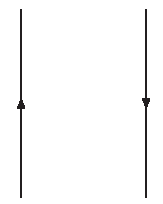
\includegraphics[scale=0.75]{holepart}
\caption{Diagrammatic representation of holes and particles, holes 
with an downward pointing arrow and particles with and upward pointing arrow.}
\label{holepart}
\end{figure}

\item The reference wavefunction, $\Phi_0,$ is represented by empty
 space.

\item Dynamical operators such as the one particle and two particle
part of the Hamiltonian are depicted by horizontal dashed lines.

\item The cluster operators are depicted by solid horizontal lines.

\item The one particle component of the Hamiltonian is represented
by a dashed interaction line capped by an $X.$


\item Representation of the cluster operators is seen in 
Fig (\ref{clusterdi}). In the diagram representing the $T_1$ amplitude there
is one incoming hole line and one outgoing particle line meeting at a solid
horizontal line.


\begin{figure}[htp]
\centering
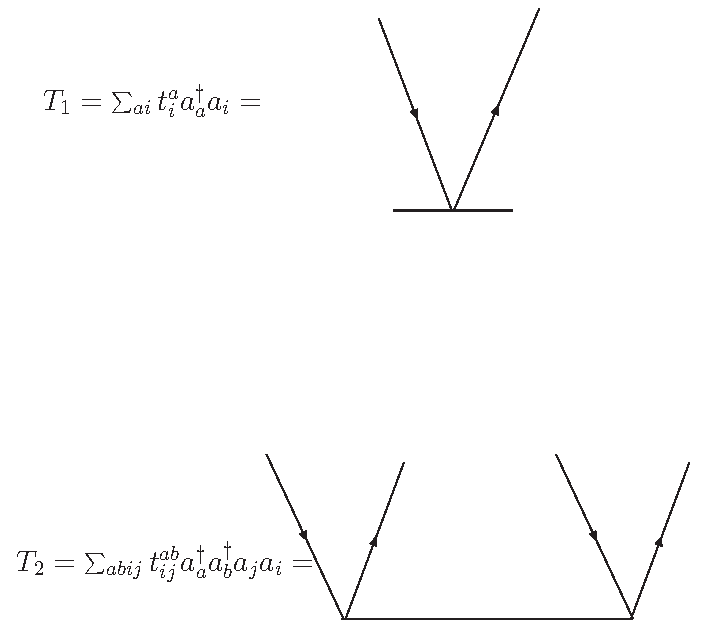
\includegraphics[scale=0.5]{clusterop}
\caption{Diagrammatic representation of the cluster operators $T_1$
and $T_2$.}
\label{clusterdi}
\end{figure}

The diagram representing $T_2$ consists of two incoming hole lines and two
outgoing particle lines. 


\item For each hole line, multiply with a factor of -1.

\item For each loop, multiply with a factor of -1

\item If there are $n$ equivalent vertices's in the diagram, multiply
with the factor $\frac{1}{n!}.$

\item For each pair of unique external hole or particle lines, multiply with
 the permutation operator $P(pq).$


\end{enumerate}

By using the above diagram rules it is possible to write diagrams
corresponding to the energy equation and amplitude equations. 

Like the diagrams for the energy equation in Eq. \eqref{lastformham}, 

\be
E=\bra{\Phi_0}H_N+H_NT_1+H_Nt_2+\frac{1}{2}H_NT^2_1+\dots \ket{\Phi_0}
\ee

can be evaluated with the above rules. The first term will not
contribute since the operator is normalized and therefore will
annihilate the vacuum state and give zero contribution.

Lets now study the second term


\be
\bra{\Phi_0}H_NT_1\ket{\Phi_0}
\label{firstendi}
\ee


Since both the incoming and outgoing states are the same there
should be now external lines, meaning that there shouldn't be 
any lines neither below or above the two horizontal operator 
lines. The $T_1$ operator stands to the right, and it's 
corresponding interaction line should then be in the bottom of 
the diagram. Only the one particle operator contributes since with a two 
particle operator it is impossible to draw a diagram with just internal 
lines. See Fig. (\ref{firstenedi}). 

%Fig. (\ref{firstenedi}) shows the diagrammatic representation of
%the energy term $\bra{\Phi_0}H_NT_1\ket{\Phi_0}.$
%Eq. \eqref{firstendi}

\begin{figure}[htp]
\centering
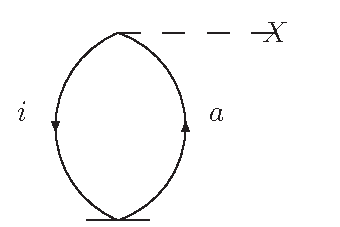
\includegraphics[scale=0.75]{firstenedi}
\caption{Diagrammatic representation of the first term in the 
ECCSD energy equation.}
\label{firstenedi}
\end{figure}






The second contributing part

\be
\bra{\Phi_0}H_NT_2\ket{\Phi_0},
\label{secendi}
\ee

has also the same ingoing as outgoing state, the same 
reasoning, with none external lines still yields. Since the 
cluster operator is the rightmost one, the interaction line 
representing it should again be at the bottom. However to this 
part only the two-particle operator of the Hamiltonian is 
contributing, something which should be reflected in the 
diagram. Fig. \ref{secndi} shows the diagram representing Eq. 
\eqref{secendi}.

\begin{figure}[htp]
\centering
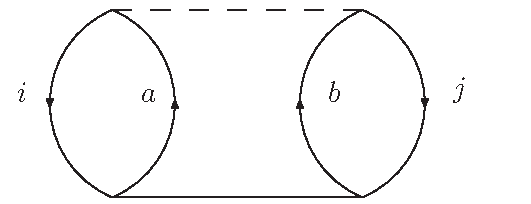
\includegraphics[scale=0.75]{secenedi}
\caption{Diagrammatic representation of the second term in the 
ECCSD energy equation.}
\label{secndi}
\end{figure}

The last part contributing to the $ECCSD$ energy equation is the
term 

\be
\frac{1}{2}\bra{\Phi_0}H_NT_1^2\ket{\Phi_0}
\label{thirdpartendi}
\ee

The interaction lines corresponding to the two cluster operators
will again have to be drawn at the bottom of the diagram, the 
difference in this diagram, Fig. (\ref{thirdenedi}), from 
Fig. (\ref{secndi}) is that the 
interaction line corresponding to the cluster operator is 
split since there are two one excitation cluster operators to
the right in Eq. \eqref{thirdpartendi} 

\begin{figure}[htp]
\centering
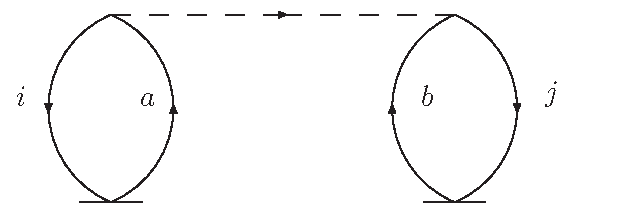
\includegraphics[scale=0.75]{thirdenedi}
\caption{Diagrammatic representation of the last term in the 
ECCSD energy equation.}
\label{thirdenedi}
\end{figure}

The cluster diagrams is computed by the same reasoning, keeping in mind that
for the $T1$ equation there should be one incoming hole line and one outgoing
particle line. The diagrams corresponding to the $T2$ equation all have two
incoming hole lines and two outgoing particle lines. The first leading term 
in the equation corresponding to $T1$ consists just of the Hamiltonian, and 
only the one particle part of it contributes. It's corresponding diagram is
depicted in Fig. (\ref{firstamplt1}).  


\begin{figure}[htp]
\centering
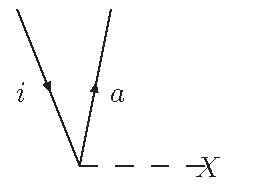
\includegraphics[scale=0.75]{firstampl}
\caption{The diagram representing the first leading term in the
$T_1$ amplitude equation.}
\label{firstamplt1}
\end{figure}

The other diagrams corresponding to $T1$ is made with the same reasoning. 
All diagrams contributing to the $T_1$ equation can be seen in Fig. (\ref{t1_eqn_diag}).\\


\begin{figure}[htp]
\centering
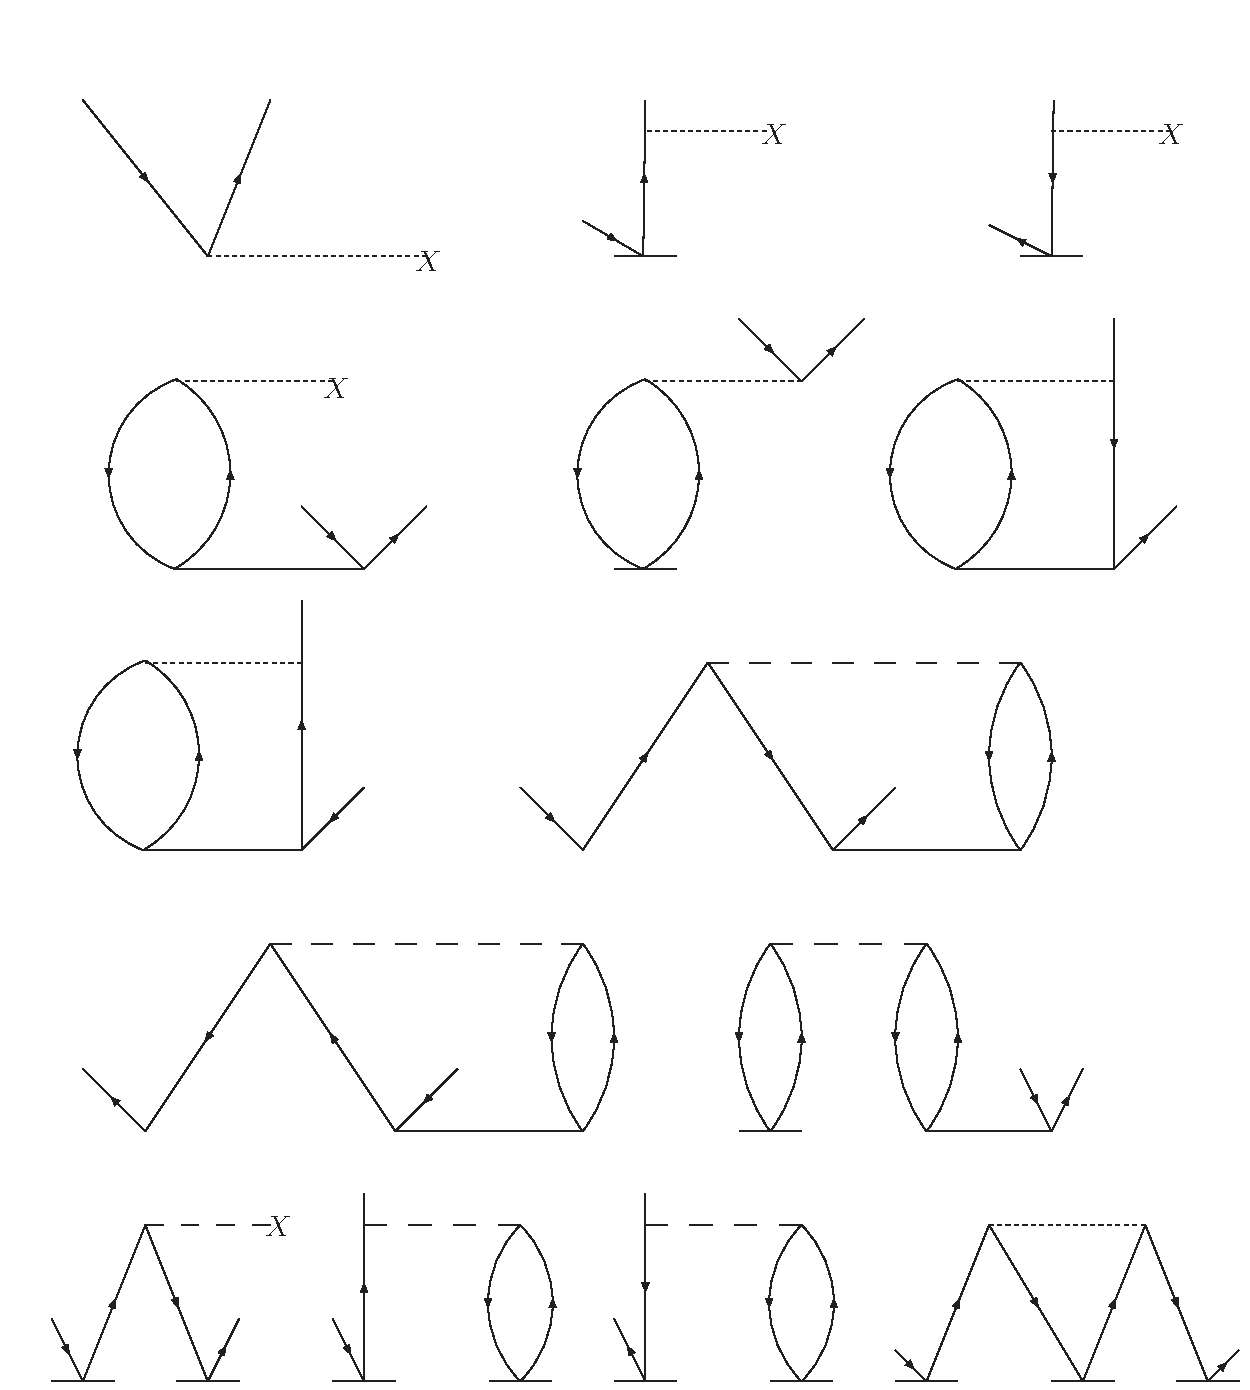
\includegraphics[scale=0.5]{t1_eqn_diag}
\caption{All diagrams contributing to the equation for solving the
$T_1$ amplitude.}
\label{t1_eqn_diag}
\end{figure}

%\clearpage

In the $T2$ amplitude diagrams there should be two incoming hole lines and
two outgoing particle lines. The first leading term consists just of the 
twoparticle operator. All the diagrams contributing to $T2$ are depicted in 
Fig. (\ref{t2_eqn_diag}).
\clearpage

\begin{figure}[htp]
\centering
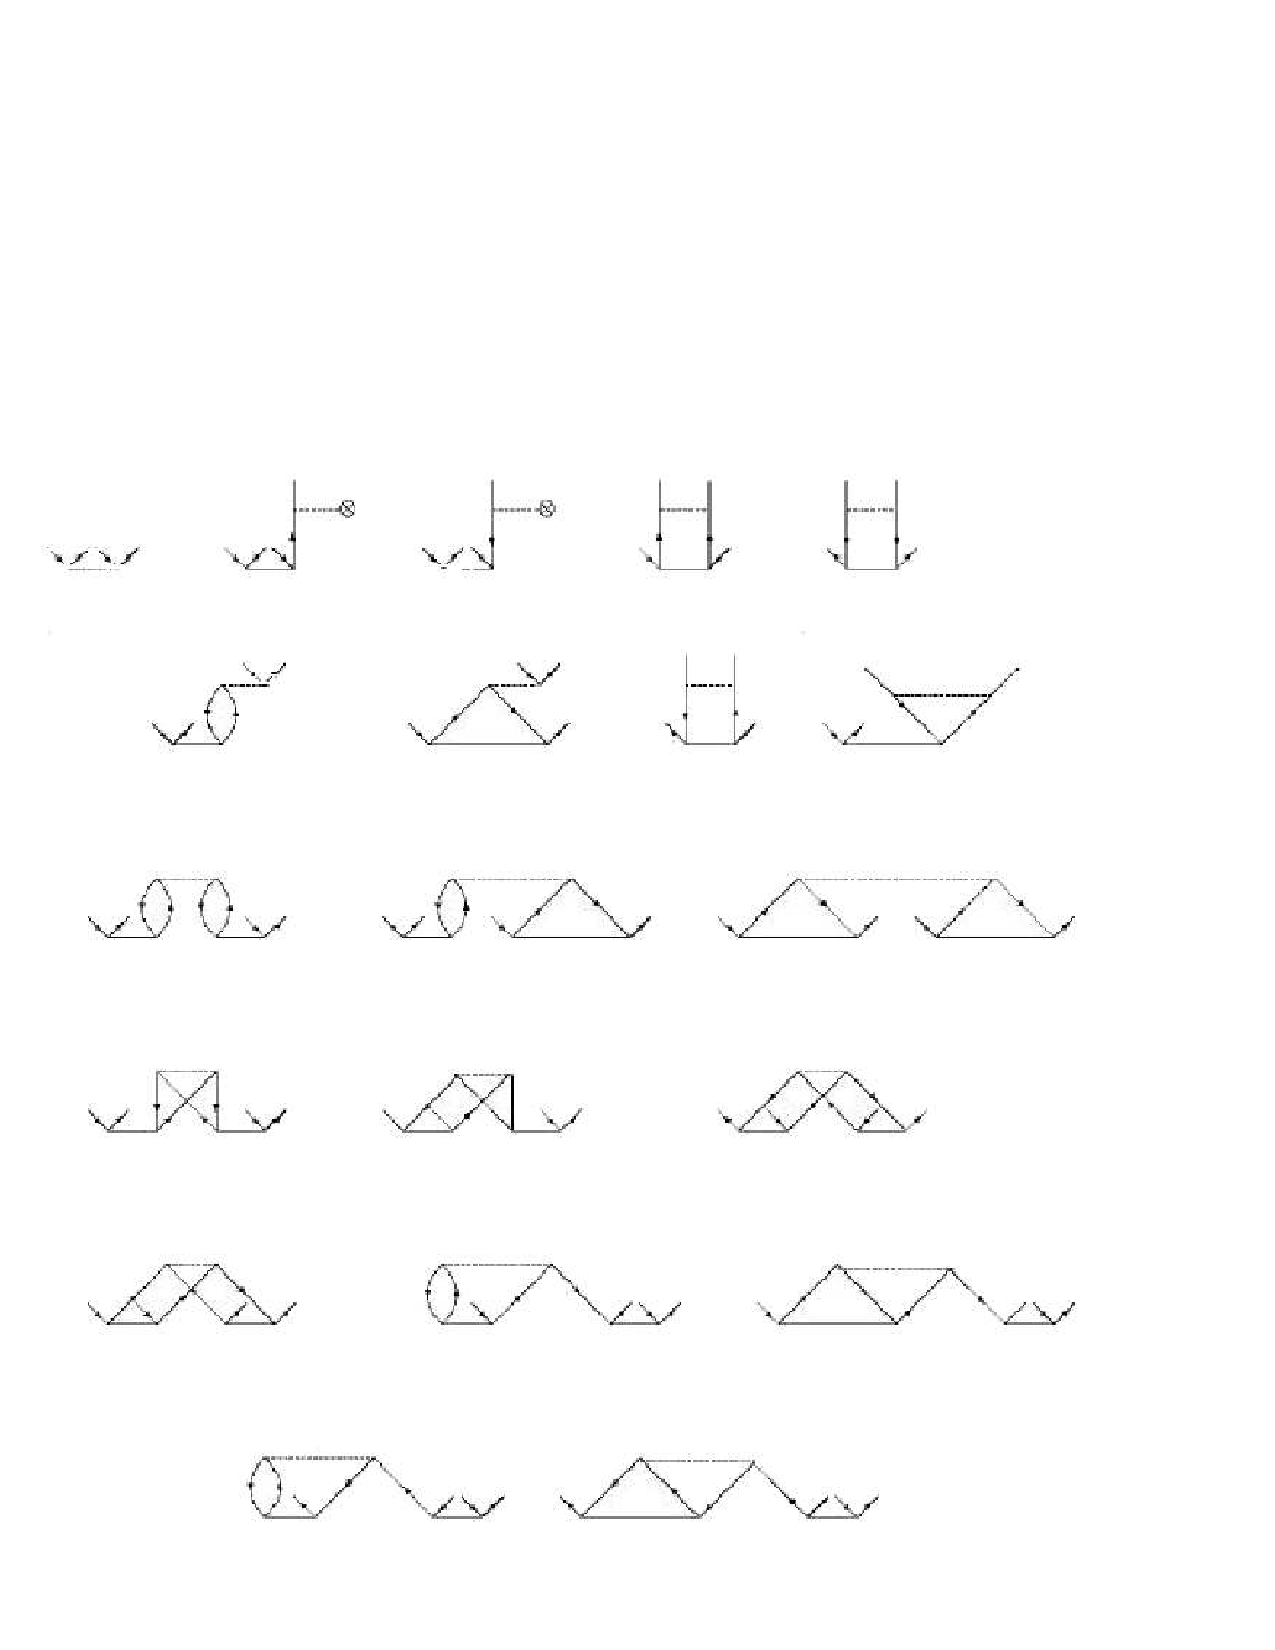
\includegraphics[scale=0.5]{CCD_diag}%{t2_eqn_diag2}
\caption{All diagrams contributing to the equation for solving the
$T_2$ amplitude.}
\label{t2_eqn_diag}
\end{figure}


\begin{figure}[htp]
\centering
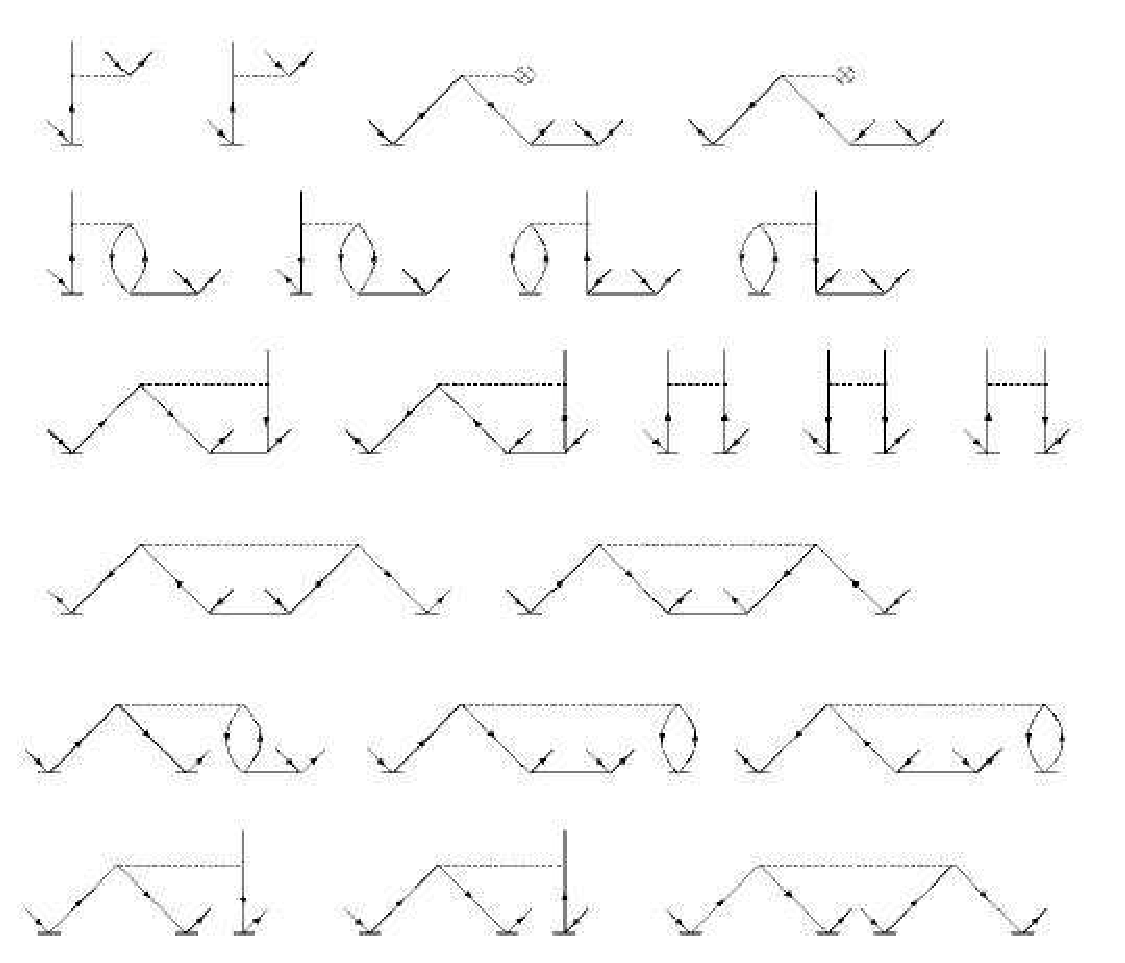
\includegraphics[scale=0.5]{CCSD_diag}%{t2_eqn_diag2}
\caption{All diagrams contributing to the equation for solving the
$T_2$ amplitude.}
\label{t2_eqn_diag}
\end{figure}


%\clearpage
To see the benefit with the diagrams, the $CCSD$ energy 
equation will now be computed from the diagrams. The total 
energy can be depicted as in Fig.(\ref{totenergydi})


\begin{figure}[htp]
\centering
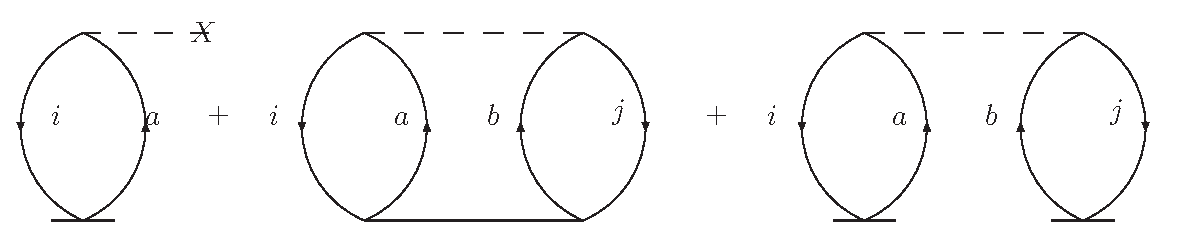
\includegraphics[width=1.0\textwidth]{energy}
\caption{The diagrams representing the total $CCSD$ 
energy.}
\label{totenergydi}
\end{figure}

The way to interpret the diagrams is from the bottom to the 
upper part, the time is upward. The ingoing states are 
represented by a ket vector and the outgoing by the dual, bra 
vector. The first figure in Fig. (\ref{totenergydi}), 
corresponding to the one particle operator should then be 
understood as

\be
\sum_{ia}\bra{i}F_N\ket{a}t^a_i=\sum_{ai}f_{ia}t^a_i,
\ee

where $f_{ia}=\bra{i}F_N\ket{a}.$ By using the above diagram 
rules to the second diagram in Fig. (\ref{totenergydi}), it's 
matrix elements become

\be
\frac{1}{4}\sum_{ijab}\bra{ij}V_N\ket{ab}t^{ab}_{ij}=\frac{1}{4}\sum_{ijab}V_{ijab}t^{ab}_{ij},
\ee

where $V_{ijab}=\bra{ij}V_N\ket{ab}.$ The last part is written 
as

\be
\frac{1}{2}\sum_{ijab}\bra{ij}V_N\ket{ab}t^a_it^b_j=\frac{1}{2}\sum_{ijab}V_{ijab}t^a_it^b_j.
\ee

After summing up the energy,  the total equation becomes

\be
\sum_{ia}f_{ia}t^a_i+\frac{1}{4}\sum_{ijab}V_{ijab}t^{ab}_{ij}
+\frac{1}{2}\sum_{ijab}V_{ijab}t^a_it^b_j,
\ee

which is exactly the same as the equation got by using Wicks 
theorem.\\ 

%The same reasoning as above for the energy equation can be done
%at the $CCSD$ amplitude equations. In this case one has to take
%in consideration that the states dealed with are excited states
%projected on the normaled ordered coupled cluster Hamiltonian 
%operated on the groundstate.
%
%The leading term in the $T_1$ amplitude  equation is $\bra{\Phi^a_i}H_N\ket{\Phi_0}$. Only the one particle operator is 
%contributing here, the corresponding diagram would be 
%
%\begin{figure}[htp]
%\centering
%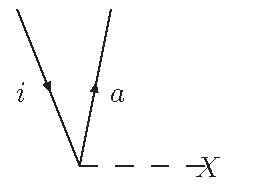
\includegraphics{firstampl}
%\caption{The diagram representing the first leading term in the
%$T_1$ amplitude equation. The interpretation is $f_{ai}$ }
%\label{firstamplt}
%\end{figure}
%
%Converting the diagram in Fig. (\ref{firstamplt}) to an equation
%would give the result $f_{ai}.$
%
%The first leading term in the $T_2$ amplitude equation is
%$\bra{\Phi^{ab}_{ij}}H_N\ket{\Phi_0},$ only the two-particle 
%operator is contributing to this part and the diagram is as is 
%shown in Fig. (\ref{secamplt})
%
%\begin{figure}[htp]
%\centering
%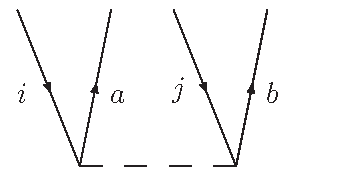
\includegraphics{secampl}
%\caption{The diagram representing the first leading term in the
%$T_2$ amplitude equation. It is representing the equation 
%$V_{ijab}$ }
%\label{secamplt}
%\end{figure}
%
%The matrix element, Fig(\ref{secamplt}), is $\bra{ab}V\ket{ij}.$


\section{Computation of the equations}

This section will treat the computational approach for solving the amplitude
equations as Eqs. \eqref{firstamplitude} and \eqref{secondamplitude}.
It is not always clear how one should approach the equations for the amplitudes. 
A first approach could be to rearrange the equations to provide a more handier form. As an example the first few terms of Eq. \eqref{firstamplitude}, could be written as

\be
0=f_{ai}+f_{aa}-f_{ii}t^a_i+\sum_c(1-\delta_{ca})f_{ac}t^c_i-\sum_k (1-\delta_{ik})f_{ik}t^a_k+\cdots
\label{firstfirstampl}
\ee

By defining 

\be
D^a_i=f_{ii}-f_{aa}
\ee

Eq. \eqref{firstfirstampl} would be rewritten as 

\be
D^a_it^a_i=f_{ai}+\sum_c(1-\delta_{ca})f_{ac}t^c_i-\sum_k(1-\delta_{ik})f_{ik}t^a_k+\cdots.
\ee

By also defining 

\be
D^{ab}_{ij}=f_{ii}+f_{jj}-f_{aa}-f_{bb}
\ee

the $T_2$ amplitude can be rewritten as

\be
D^{ab}_{ij}t^{ab}_{ij}=\bra{ab}V\ket{ij}+P(ab)\sum_c(1-\delta_{bc})f_{bc}t^{ac}_{ij}-P(ij)\sum_{k}(1-\delta_{kj})f_{kj}t^{ab}_{ik}+\cdots
\ee

The equations above have to be solved iteratively. A starting point for $t^a_i$ and $t^{ab}_{ij}$ may be obtained by setting all of the amplitudes on the right-hand side to zero. The initial guess for the amplitudes are then

\be
t^a_i=f_{ai}/D^a_i,
\ee 

for the $T_1$ amplitude and 

\be
t^{ab}_{ij}=\bra{ab}V\ket{ij}/D^{ab}_{ij}
\ee

for the $T_2$ amplitude.\\

 These initial guesses have to be inserted on the right-hand side of the 
equations and then subsequently used to obtain new 
amplitudes. This process is continued until an explicit convergence is 
reached.

We saw in Eqs. \eqref{firstamplitude} and \eqref{secondamplitude} that there
are many diagrams contributing to the amplitude equations, as many diagrams
as terms in the equations. It requires a lot of time computing all these
diagrams separately. By saving a great amount of computing time the 
amplitude diagrams are factorized. The coupled cluster diagrams can be 
factorized in contrast to the diagrams in perturbation theory since the 
first ones do not have any denominators in their's expressions. By notice 
that some diagrams are similar in the sense that they have the same factors.
Instead of computing the same factors several times, we compute it once and
multiply it with the corresponding terms, as explained by \cite{bartlett:291}. In this work the factorization used is the same as the one used by \cite{hagen:034302}.


 % coupled.tex

\appendix
\chapter{Diagram rules} \label{diagramregler}

\begin{enumerate}
\item There are $n+1$ vertices, one vertice for each time, with the ordring
$t<t_1<t_2 < \cdots < t_n.$ Each vertex/interaction is represented by a 
dashed line, as in Fig.(\ref{forsteordendiagram}). 

\item Lines with upward pointing arrows are particles and lines with 
downward pointing arrows are holes. Lines starting and ending at the same 
vertex ate holes.

\item Each vertex gives a factor $\frac{1}{2}V_{\alpha\beta\gamma\delta}.$

\item There is an overall sign $(-1)^{n_h+n_l},$ where $n_h$ is the number
of hole lines and $n_l$ is the number of fermion loops.

\item For each interval between two successive vertices there are an energy
factor 

\beq
\left[\sum_h \epsilon_h - \sum_p \epsilon_p \right]^{-1}
\eeq

Where the sum over $h$ is over all hole lines in the intervall and the sum 
over $p$ is over all particle lines in the intervall.

\item For each pair of lines that begins at the same interaction line and 
end at the same interaction line gives a factor $\frac{1}{2}.$

\item All the above factors have to be multiplied. Sum over all the labels 
of fermion lines. 











\end{enumerate}

\bibliographystyle{h-physrev3}
\bibliography{bibliografi.bib}
%\bibliography{mylib.bib}
\end{document}
